\setchapterpreamble[u]{\margintoc}
\chapter{Mecánica Lagrangiana}
\labch{Part}

\section{Dinámica Lagrangiana}
En este capítulo mostramos cómo se pueden reescribir las ecuaciones de movimiento en la variedad de configuración adecuada, de forma que las restricciones se tengan en cuenta desde el principio. El resultado es la formulación lagrangiana de la dinámica (las ecuaciones de movimiento se denominan entonces ecuaciones de Lagrange). Hay que subrayar que el contenido físico de las ecuaciones de Lagrange es el mismo que el de las de Newton. Pero además de ser lógicamente más atractiva, la formulación de Lagrange tiene varias ventajas importantes.

Quizá la primera ventaja evidente es que la formulación lagrangiana es más fácil de aplicar a sistemas dinámicos distintos del más simple. Además, pone de manifiesto la conexión entre las leyes de conservación e importantes propiedades de simetría de los sistemas dinámicos. De gran importancia es que las ecuaciones de Lagrange pueden derivarse de un principio variacional, un método que resulta ser extremadamente general y aplicable en muchas ramas de la física. Una de las razones para estudiar mecánica clásica es comprender la formulación lagrangiana, ya que muchas ecuaciones de la física se formulan convencionalmente en términos lagrangianos y muchas leyes de conservación se entienden también en términos lagrangianos, a través de su conexión con las simetrías.

\subsection{Espacio de configuración}
(54-70)

En esta sección cambiamos las coordenadas cartesianas por otras más útiles para tratar sistemas dinámicos. Las nuevas coordenadas se eligen de un modo que depende del sistema dinámico concreto para el que se van a utilizar (pero se denominan, no obstante, coordenadas generalizadas); se adaptan a ese sistema y son coordenadas más o menos naturales para él. Las propiedades del sistema que determinan la elección son geométricas: son el número de libertades y la forma, o topología, de la región en la que el sistema es libre de moverse (por ejemplo, si es una esfera o un plano inclinado). Esta región está determinada por las restricciones impuestas sobre el sistema; se llama el espacio de configuraciones $\mathbb{Q}$. Las nuevas coordenadas, llamadas $q^{\alpha}$, estarán en $\mathbb{Q}$, y su número será el número de libertades, que es también la dimensión de $\mathbb{Q}$. En esta sección hacemos dos cosas 
\begin{enumerate}
  \item Explicar la idea del colector de configuración
  \item Describir el cambio de las coordenadas cartesianas a las $q^{\alpha}$
\end{enumerate}

\subsection{Lagrangianos equivalentes}



Aunque la función Lagrangiana determina las ecuaciones de movimiento de manera única, las ecuaciones de movimiento no determinan la Lagrangiana de manera única. Es decir, dos Lagrangianas que son diferentes pueden conducir a ecuaciones de movimiento que son las mismas. Por ejemplo, sea $L_{1}$ y $L_{2}$ dos funciones Lagrangianas tales que las ecuaciones de movimiento obtenidas de ellas son exactamente las mismas. Entonces se puede demostrar que existe una función $\Phi$ en $\mathbb{Q}$ tal que 

\[
L_{1}-L_{2}=\frac{d \Phi}{d t}.
\]

Para probar esta afirmación, debemos explicar lo que se entiende por "exactamente las mismas". 
\begin{proof}
  Para este propósito, consideremos las $2 n$ funciones $\Lambda_{j \alpha}$, donde $j=1,2$, y $\alpha=1, \ldots, n$, definidas por

\[
\frac{d}{d t} \frac{\partial L_{j}}{\partial \dot{q}^{\alpha}}-\frac{\partial L_{j}}{\partial q^{\alpha}} \equiv \Lambda_{j \alpha}(q, \dot{q}, \ddot{q}, t)
\]

de modo que las ecuaciones de Lagrange se pueden escribir como 

\[
\Lambda_{j \alpha}(q, \dot{q}, \ddot{q}, t)=0.
\]

Entonces, decir que las ecuaciones de movimiento son exactamente las mismas es decir que las dos funciones son iguales. En otras palabras, 

\[
\Lambda_{1 \alpha}=\Lambda_{2 \alpha} \tag{2.30}
\]

identicamente, para cada $\alpha$. Ahora procedemos a probar la afirmación, pero solo para un grado de libertad (es decir, para $n=1$), dejando el caso general para el Problema 4. Para $n=1$, el índice $\alpha$ puede ser eliminado de las ecuaciones. Escribimos $\psi=L_{1}-L_{2}$. Entonces, la Ec. (2.29) se puede usar para escribir (2.30) en la forma 

\[
\Lambda_{1}-\Lambda_{2} \equiv \frac{\partial^{2} \psi}{\partial \dot{q}^{2}} \ddot{q}+\frac{\partial^{2} \psi}{\partial q \partial \dot{q}} \dot{q}+\frac{\partial^{2} \psi}{\partial \dot{q} \partial t}-\frac{\partial \psi}{\partial q}=0 \tag{2.31}
\]

Debido a que $L_{1}$ y $L_{2}$ son funciones solo de $q, \dot{q}$ y $t$, también lo es $\psi$, y por lo tanto el único lugar donde $\ddot{q}$ aparece en (2.31) es donde se ve multiplicando el primer término. Pero (2.31) debe ser cierto para todos los valores de $q, \dot{q}, \ddot{q}, t$. Por lo tanto, el coeficiente de $\ddot{q}$ debe anularse: $\frac{\partial^{2} \psi}{\partial \dot{q}^{2}}=0$. Esto significa que $\psi$ es lineal en $\dot{q}$:

\[
\psi=\dot{q} F(q, t)+G(q, t) \tag{2.32}
\]

Esto y un poco de álgebra pueden usarse para transformar (2.31) en 

\[
\frac{\partial F}{\partial t}-\frac{\partial G}{\partial q}=0 \tag{2.33}
\]

Esto es solo la condición de integrabilidad para el par de ecuaciones 

\[
F=\frac{\partial \Phi}{\partial q} \quad \text{y} \quad G=\frac{\partial \Phi}{\partial t} \tag{2.34}
\]

Es decir, (2.33) es la condición de que exista una función local $\Phi(q, t)$ que haga posible escribir $F$ y $G$ localmente en la forma de (2.34). Cuando se escriben de esta manera, (2.32) se convierte en 

\[
\psi=\dot{q} \frac{\partial \Phi}{\partial q}+\frac{\partial \Phi}{\partial t} \equiv \frac{d \Phi}{d t}
\]

como se afirmó.
\end{proof}

La énfasis en la localidad aquí es para advertir al lector que puede no ser posible encontrar una función univaluada $\Phi(q, t)$ en todo $\mathbb{Q}$. Tales cuestiones se discutirán más a fondo más adelante.

Lo que acabamos de probar (o más bien lo que se prueba en el Problema 4) significa que si una Lagrangiana se cambia al agregar la derivada temporal de una función, las ecuaciones de movimiento no se verán alteradas. Sin embargo, esto no significa que las Lagrangianas que producen la misma dinámica deben diferir necesariamente por una derivada total en el tiempo. Por ejemplo, 

\[
L_{a}=\dot{q}^{1} \dot{q}^{2}-q^{1} q^{2} 
\]

y 

\[
L_{b}=\frac{1}{2}\left[\left(\dot{q}^{1}\right)^{2}+\left(\dot{q}^{2}\right)^{2}-\left(q^{1}\right)^{2}-\left(q^{2}\right)^{2}\right]
\]

producen la misma dinámica, pero no difieren por una derivada total en el tiempo.



\subsection{Coordenadas independientes}


Las ecuaciones de Lagrange se derivaron sin especificar de ninguna manera los coordenadas generalizadas particulares utilizadas en $\mathbb{Q}$, y por lo tanto, son válidas en un sistema de coordenadas tanto como en otro. Esta es una propiedad importante y útil de la formulación lagrangiana (ver la Sección 2.2.4 para un ejemplo de su utilidad). Para observarlo en detalle, sea $q^{\prime 2}(q, t)$ un nuevo conjunto de coordenadas generalizadas, en cuyo caso las funciones deben ser invertibles: existen $q^{\omega}(q^{\prime}, t)$. Lo que esto significa físicamente es que es posible escribir las trayectorias de las partículas en términos de $q^{\prime \alpha}$ así como en términos de $q^{\alpha}$, y cuando se conocen en términos de un conjunto, se pueden calcular en términos del otro. Cuando se conocen los $q^{\alpha}(q^{\prime}, t)$, también se conocen los $\dot{q}^{\alpha}(q^{\prime}, \dot{q}^{\prime}, t)$:

\begin{DispWithArrows}[displaystyle, format=c]
\dot{q}^{\alpha}\left(q^{\prime}, \dot{q}^{\prime}, t\right)=\frac{\partial q^{\alpha}\left(q^{\prime}, t\right)}{\partial q^{\prime \beta}} \dot{q}^{\prime \beta}+\frac{\partial q^{\alpha}\left(q^{\prime}, t\right)}{\partial t} \tag{2.35}
\end{DispWithArrows}


La Lagrangiana es una función de $2 n+1$ variables: las $n$ coordenadas generalizadas, sus $n$ derivadas temporales, y el tiempo. Esto significa que $L$ asigna un número real (el valor de la función) a cada conjunto de $2 n+1$ números (los valores de las variables). Pero el conjunto de $2 n+1$ números describe el estado físico del sistema dinámico. Por lo tanto, la función Lagrangiana asigna un número real no a cada conjunto de $2 n+1$ números, sino al estado físico en sí. Cuando se realiza una transformación de coordenadas, el mismo estado físico del sistema se describe mediante un conjunto diferente de $2 n+1$ números. Dado que el estado no cambia, la función Lagrangiana debe asignar el mismo valor real a este conjunto transformado de $2 n+1$ números.

Ahora lo hacemos explícito matemáticamente. Suponga que se da una función Lagrangiana $L(q, \dot{q}, t)$ en las coordenadas originales, sin primar. Se puede escribir en términos de las coordenadas primadas simplemente sustituyendo las expresiones conocidas para $q^{\alpha}$ y $\dot{q}^{\alpha}$ en términos de $q^{\prime \beta}$ y $\dot{q}^{\prime \beta}$. El resultado será una nueva función Lagrangiana (transformada) $L^{\prime}$ de las coordenadas primadas, diferente de $L$. Es decir, $L^{\prime}\left(q^{\prime}, \dot{q}^{\prime}, t\right)$ está definida por

\begin{DispWithArrows}[displaystyle, format=c]
L^{\prime}\left(q^{\prime}, \dot{q}^{\prime}, t\right) \equiv L\left(q\left(q^{\prime}, t\right), \dot{q}\left(q^{\prime}, \dot{q}^{\prime}, t\right), t\right) \equiv L(q, \dot{q}, t) \tag{2.36}
\end{DispWithArrows}


la igualdad surge de lo que se ha dicho: las variables primadas y no primadas describen el mismo estado físico del sistema. Entonces, como se muestra en el Problema 3, las ecuaciones de Lagrange (2.28) implican

\begin{DispWithArrows}[displaystyle, format=c]
\frac{d}{d t} \frac{\partial L^{\prime}}{\partial \dot{q}^{\prime \prime}}-\frac{d L^{\prime}}{d q^{\prime \alpha}}=0 \tag{2.37}
\end{DispWithArrows}


Debido a que esta ecuación y (2.28) son igualmente válidas, se dice que las ecuaciones de Lagrange son independientes de las coordenadas (o covariantes bajo transformaciones de coordenadas). Pero entonces, estas ecuaciones están haciendo una afirmación que no depende de las coordenadas, y los específicos $q^{\alpha}$ o $q^{\prime 2}$ que aparecen en ellas desempeñan un papel no esencial, completamente auxiliar. Debería entonces haber una manera de escribir estas ecuaciones diferenciales sobre el conjunto de configuraciones de tal manera que las coordenadas no aparezcan.



\todo{Aunque realmenete luego siempre volvemos a las coordenadas espaciales en la práctica}
\subsection{Condición Hessiana}

Tanto en las formulaciones de Lagrange como en las de Newton, las ecuaciones del movimiento son de segundo orden. Estas ecuaciones describen cómo evoluciona el estado de un sistema prescribiendo la aceleración basada en el estado actual, es decir, la posición y la velocidad del sistema. La integración de estas ecuaciones, comenzando desde las condiciones iniciales, nos permite determinar el comportamiento del sistema en tiempos futuros.

Las ecuaciones de Lagrange, que a menudo son más generales y se adaptan mejor a sistemas con restricciones, se pueden reescribir en la siguiente forma matricial:

\[
\frac{\partial^2 L}{\partial \dot{q}^\beta \partial \dot{q}^\alpha} \ddot{q}^\beta = G_\alpha (q, \dot{q}, t)
\]

donde $ G_\alpha $ y las segundas derivadas parciales en el lado izquierdo son funciones de $ (q, \dot{q}, t) $, que se pueden calcular una vez que se conoce el Lagrangiano. Los términos $ \ddot{q}^\beta \left(t_0\right) $ se pueden encontrar insertando los valores iniciales $ q \left(t_0\right) $ y $ \dot{q} \left(t_0\right) $ en las expresiones para $ G_\alpha $ y $ \frac{\partial^2 L}{\partial \dot{q}^\alpha \partial \dot{q}^\beta} $, los cuales forman una columna numérica y una matriz numérica. Luego, aplicando la inversa de la matriz a ese vector se obtienen las aceleraciones iniciales. Para que esto funcione, la matriz Hessiana $ \frac{\partial^2 L}{\partial \dot{q}^\alpha \partial \dot{q}^\beta} $ debe ser no singular. Por lo tanto, siempre asumimos (a menos que se indique explícitamente lo contrario) que:

\[
\operatorname{det}\left(\frac{\partial^2 L}{\partial \dot{q}^\alpha \partial \dot{q}^\beta}\right) \neq 0
\]

Esto se conoce como la condición Hessiana.\todo{Esta condición asegura que las ecuaciones de Newton son equivalentes al Lagrangiano dado un sistema}

\subsection{Conservación de la energía}
La diferencia entre la función lagrangiana usual $L = T - V$ y la energía $E = T + V$ radica únicamente en el signo de $V$. ¿Existe algún método general para calcular $E$ a partir del conocimiento de $L$? Para una partícula única en coordenadas cartesianas, siempre que $V$ sea independiente de la velocidad $\dot{x}$ (es decir, siempre que $\partial V / \partial \dot{x}^{\alpha} = 0$)\todo{También vale $\pdv{V}{\dot{x}^{a}}=cte$}, esto puede hacerse fácilmente. Escribimos $T = \frac{1}{2} m \dot{x}^{2}$; luego,

$$
\dot{x}^{\alpha \alpha} \frac{\partial L}{\partial \dot{x}^{\alpha}} - L = \dot{x}^{\alpha} \frac{\partial T}{\partial \dot{x}^{\dot{\alpha}}} - T + V = T + V = E \tag{2.38}
$$

Ahora tomamos este enfoque para generalizar de una partícula a varias coordenadas generalizadas. El análogo de $E$, tal como se define en (2.38), es la variable dinámica

$$
h \equiv E(q, \dot{q}) \equiv \dot{q}^{\alpha} \frac{\partial L}{\partial \dot{q}^{\alpha}} - L \tag{2.39}
$$

Este $E$ generalizado es un candidato para la energía total en general. Primero verificamos su conservación:

$$
\dot{E} = \frac{d}{d t}\left[\dot{q}^{\alpha} \frac{\partial L}{\partial \dot{q}^{\alpha}} - L\right] = \ddot{q}^{\alpha} \frac{\partial L}{\partial \dot{q}^{\alpha}} + \dot{q}^{\alpha} \frac{d}{d t} \frac{\partial L}{\partial \dot{q}^{\alpha}} - \ddot{q}^{\alpha} \frac{\partial L}{\partial \dot{q}^{\alpha}} - \dot{q}^{\alpha} \frac{\partial L}{\partial q^{\alpha}} - \frac{\partial L}{\partial t}
$$

Los primeros y terceros términos en el lado derecho se cancelan, y las ecuaciones de Lagrange implican que los segundos y cuartos términos también se cancelan; así que

$$
\frac{d E}{d t} = -\frac{\partial L}{\partial t} \tag{2.40}
$$

Esto significa que si $L$ es independiente del tiempo, $E$ se conserva, es decir,

$$
\frac{\partial L}{\partial t} = 0 \Rightarrow \frac{d E}{d t} = 0 \tag{2.41}
$$

En otras palabras, si $\partial L / \partial t = 0$, entonces $E$ es una constante del movimiento, como la energía. Pero aún no hemos establecido si $E$ es de hecho la energía $T + V$. Para hacerlo, ahora calculamos $T$ explícitamente en coordenadas generalizadas:

$$
T = \frac{1}{2} \sum_{t} m_{l} v_{t}^{2} = \frac{1}{2} \sum_{t} m_{l} \left[\frac{\partial \mathbf{x}_{l}}{\partial q^{\alpha}} \dot{q}^{\alpha} + \frac{\partial \mathbf{x}_{t}}{\partial t}\right] \cdot \left[\frac{\partial \mathbf{x}_{t}}{\partial q^{\gamma}} \dot{q}^{\gamma} + \frac{\partial \mathbf{x}_{t}}{\partial t}\right]
$$

donde

$$
T = a(q, t) + A_{\alpha}(q, t) \dot{q}^{\alpha} + T_{\alpha \beta}(q, t) \dot{q}^{\alpha} \dot{q}^{\beta}
$$

Los coeficientes son

$$
a = \frac{1}{2} \sum_{i} m_{i} \frac{\partial \mathbf{x}_{t}}{\partial t} \cdot \frac{\partial \mathbf{x}_{t}}{\partial t}
$$

$$
A_{\alpha} = \sum_{i} m_{i} \frac{\partial \mathbf{x}_{t}}{\partial t} \cdot \frac{\partial \mathbf{x}_{t}}{\partial q^{\alpha}} \tag{2.42}
$$

$$
T_{\alpha \beta} = \frac{1}{2} \sum_{i} m_{i} \frac{\partial \mathbf{x}_{t}}{\partial q^{\alpha}} \cdot \frac{\partial \mathbf{x}_{t}}{\partial q^{\beta}}
$$

Son funciones de $q$ y $t$, pero no de $\dot{q}$. Por lo tanto, $T$ es una función cuadrática de $\dot{q}^{\alpha}$, pero no es en general una función cuadrática homogénea.

Ahora explicamos la homogeneidad. Una función $f$ de $k$ variables $z_{1}, \ldots, z_{k}$ es homogénea de grado $\lambda$ si y solo si, para todo $a > 0$,

$$
f(a z_{1}, \ldots, a z_{k}) = a^{\lambda} f(z_{1}, \ldots, z_{k})
$$

Por ejemplo, $z_{1} + 7 z_{1} z_{2} + 3 (z_{2})^{2}$ es cuadrática, y $7 z_{1} z_{2} + 3 (z_{2})^{2}$ es homogénea cuadrática. Usaremos frecuentemente el teorema de Euler sobre funciones homogéneas: si $f$ es homogénea de grado $\lambda$, entonces

$$
z_{t} \frac{\partial f}{\partial z_{t}} = \lambda f
$$

La razón por la que la homogeneidad de $T$ es importante es que (suponemos que $\partial V / \partial \dot{q}^{\alpha} = 0$ y $\partial V / \partial t = 0$), el teorema de Euler implica que

$$
E = \dot{q}^{\alpha} \frac{\partial T}{\partial \dot{q}^{\alpha}} - L = 2 T - T + V = T + V
$$
\todo{Puede ser $L$ si como está en la otra nota $\pdv{V}{\dot{x}^{a}}=cte$ o 0}
Por lo tanto, la homogeneidad garantiza que $E$ es la energía. Entonces, ¿en qué condiciones es $T$ homogénea cuadrática en $\dot{q}$? Según la Ecuación (2.42), si las $\mathbf{x}_{t}$ son funciones independientes del tiempo de $q$, entonces $a = 0$ y $b_{\alpha} = 0$, y $T$ es homogénea cuadrática en $\dot{q}^{\alpha}$ (puede seguir siendo una función de $q^{\text{e}}$, pero no de $t$).

Por lo tanto, si $L = T - V$ es independiente del tiempo, el potencial $V$ es independiente de $\dot{q}$ y la transformación de coordenadas cartesianas a coordenadas generalizadas es independiente del tiempo, entonces $E$ es la energía. Aunque esto puede parecer muchas suposiciones arbitrarias, es una de las situaciones más comunes. Por lo tanto, la Ecuación (2.41) establece que bajo estas condiciones la energía se conserva. Nótese que la variable dinámica $E$ se conserva bajo la única condición de que $L$ sea independiente del tiempo, pero esta única condición no garantiza que $E$ sea la energía.
\subsection{Trayectorias y variaciones infinitesimales}
\subsubsection{Las velocidades no están en $\mathbb{Q}$}
Volvemos ahora a la discusión de las ecuaciones de Lagrange en la forma de las Ecs. (2.28) o (2.29), a saber

\begin{DispWithArrows}[format=c, displaystyle]
  \frac{d}{d t} \frac{\partial L}{\partial \dot{q}^{\alpha}}-\frac{\partial L}{\partial q^{\alpha}}=0 \tag{2.28}

\end{DispWithArrows}
  o
  \begin{DispWithArrows}[format=c, displaystyle]
    \frac{\partial^{2} L}{\partial \dot{q}^{\beta} \partial \dot{q}^{\alpha}} \ddot{q}^{\beta}+\frac{\partial^{2} L}{\partial q^{\beta} \partial \dot{q}^{\alpha}} \dot{q}^{\beta}+\frac{\partial^{2} L}{\partial t \partial \dot{q}^{\alpha}}-\frac{\partial L}{\partial q^{\alpha}}=0 . \tag{2.29}
  \end{DispWithArrows}

    Hasta ahora, aunque hemos mencionado superficialmente el espacio de fases de velocidad, hemos tratado estas ecuaciones como un conjunto de ecuaciones diferenciales de segundo orden en la variedad de configuración $Q$. En esta sección extendemos la idea del espacio de fases de velocidad a la variedad de fases de velocidad $\mathbf{T} \mathbb{Q}$. En el proceso, mostraremos la importancia de las variedades al mostrar cómo las propiedades de los sistemas dinámicos generales se reflejan en la estructura de la variedad de $T \mathbb{Q}$.

    Algunas de estas propiedades se ilustran comparando dos sistemas diferentes, cada uno formado por dos partículas materiales. En el primer sistema, las dos partículas se mueven en el espacio euclidiano tridimensional ordinario $\mathbb{E}^{3}$. La diferencia $\mathbf{v}{1}-\mathbf{v}{2}$ entre sus velocidades es un vector en $\mathbb{E}^{3}$ (que puede moverse a cualquier punto en $\mathbb{E}^{3}$) y tiene un significado físico claro: es la velocidad relativa de los dos puntos. En el segundo sistema, las dos partículas se mueven en la superficie bidimensional de una esfera $\mathbb{S}^{2}$. El vector velocidad de cada partícula es tangente a la esfera: sale de la esfera y se extiende hacia el $\mathbb{E}^{3}$ en el que está incrustada la esfera. Todos los vectores de velocidad posibles en cualquier punto de la esfera se encuentran en el plano tangente a la esfera en ese punto: abarcan ese plano (el plano es un espacio vectorial bidimensional). Por mucho que queramos discutir el movimiento en $\mathbb{S}^{2}$ únicamente en términos de objetos en $\mathbb{S}^{2}$ mismo, nos vemos obligados a salir de $\mathbb{S}^{2}$ hacia el plano tangente, de hecho, hacia el conjunto de todos los planos tangentes en todos los puntos de la esfera. Y aun así no es suficiente, ya que la diferencia entre los vectores velocidad en dos puntos diferentes no se encuentra en ninguno de los planos tangentes, y aunque esta diferencia es la velocidad relativa de los dos puntos en $\mathbb{E}^{3}$, no representa nada físico que pueda describirse simplemente en términos de $\mathbb{S}^{2}$ mismo. Esto es ciertamente diferente del primer sistema de dos partículas en $\mathbb{E}^{3}$.
    
    En este ejemplo no es muy importante tratar el movimiento únicamente en términos de $\mathbb{S}^{2}$; puede tratarse en el $\mathbb{E}^{3}$ en el que está incrustado $\mathbb{S}^{2}$. Sin embargo, en muchos otros sistemas dinámicos, no hay un espacio de mayor dimensión disponible fácilmente. Por ejemplo, el doble péndulo de la Fig. 2.3(e) no tiene un espacio físico obvio en el que incrustar la variedad de configuración de cuatro dimensiones. Aunque se puede demostrar que $\mathbb{S}^{2} \times \mathbb{S}^{2}$, como todas las variedades que tratamos en este libro, puede incrustarse en algún $\mathbb{E}^{n}$, este $\mathbb{E}^{n}$ no es obvio y no tiene un significado físico particular. Incluso su dimensión $n$ no es evidente.
    
    Por razones como esta, es importante mantener la discusión general intrínseca a la propia variedad de configuración, sin introducir espacios de mayor dimensión excepto en formas que surgen de la propia $\mathbb{Q}$. Se verá que $\mathbf{T} \mathbb{Q}$ está construida de esta manera, a partir de la propia $\mathbb{Q}$.
    
    En un espacio vectorial, la dinámica es relativamente fácil de tratar, principalmente porque los vectores velocidad son similares a los vectores de posición. Sin embargo, en las variedades surgen problemas del tipo que se encuentran en el ejemplo de $\mathbb{S}^{2}$, y los vectores deben discutirse en términos de espacios tangentes, los análogos de los planos tangentes de $\mathbb{S}^{2}$. Como en $\mathbb{S}^{2}$, no hay una manera inmediatamente evidente de comparar vectores en diferentes puntos, por lo que las velocidades relativas presentan problemas. Uno de los primeros obstáculos al tratar con dinámica en variedades es, por lo tanto, encontrar una forma coherente de tratar los vectores tangentes. Otra dificultad será encontrar una manera coherente de abordar una cuestión que ya encontramos en algunos de los ejemplos de la variedad de configuración de la Sección 2.1: en general, es imposible encontrar un sistema de coordenadas que cubra una variedad, a diferencia de un espacio vectorial, sin puntos con valores múltiples.
    
    \subsubsection{}
    En $TQ$ (a diferencia de $Q$), las ecuaciones de Lagrange son un conjunto de ecuaciones diferenciales de primer orden (a diferencia de segundo orden): su solución en coordenadas generalizadas son las $2n$ funciones $q^{\alpha}(t), \dot{q}^{\alpha}(t)$, con las $\ddot{q}^{\beta}$ que aparecen en (2.29) interpretadas como las derivadas de $\dot{q}^{\beta}$ con respecto al tiempo $t$. Puede parecer que hay $2n$ funciones que deben encontrarse a partir de las $n$ ecuaciones de Lagrange, pero en realidad hay otras $n$ ecuaciones, también de primer orden: \begin{DispWithArrows}[displaystyle, format=c] \dot{q}^{\alpha} = \frac{d q^{\alpha}}{d t} \tag{2.79} \end{DispWithArrows}

Por lo tanto, hay $2n$ ecuaciones para las $2n$ funciones. Las ventajas de ver el sistema dinámico como un conjunto de ecuaciones de primer orden en $T \mathbb{Q}$ son las discutidas en relación con el espacio de fase de velocidades en el Capítulo 1.

Como demostración, construimos el retrato de fase del péndulo plano de la Fig. 2.3(b) en su haz tangente. El retrato de fase es similar a la Fig. 1.5(b), excepto que la variedad de fase es ahora un cilindro en lugar de un plano: las líneas $\theta = \pi$ y $\theta = -\pi$ están identificadas (recuerda que $q$ se llama $\theta$ en este ejemplo). La energía potencial es un múltiplo de $\cos \theta$, como lo fue en el ejemplo de la Ecuación (1.49), y la energía cinética es un múltiplo de $\dot{\theta}^{2}$: 
\begin{DispWithArrows}[displaystyle, format=c] 
  E = \frac{1}{2} m l^{2} \dot{\theta}^{2} - m g \cos \theta \end{DispWithArrows}

Esto es lo mismo que la Ecuación (1.50) pero en notación diferente. Por lo tanto, dondequiera que esta expresión para $E$ sea válida (es decir, para el rango de $\theta$ de $-\pi$ a $\pi$), el retrato de fase será el mismo que el obtenido de la Ecuación (1.50). La Figura 2.11 muestra este retrato de fase dibujado en dos vistas del cilindro. Los puntos de equilibrio elípticos e hiperbólicos y una separatriz se reconocen comparando esta figura con la del Capítulo 1. El punto elíptico corresponde al péndulo colgando hacia abajo, y el punto hiperbólico a su equilibrio vertical. La separatriz consta de tres órbitas distintas.

Considera un valor fijo de $\theta$. Como sería cierto si $\mathbb{Q}$ fuera una línea infinita, en la variedad de configuración circular $\mathbb{Q} = \mathbb{S}^{1}$ hay muchas trayectorias que pasan por $\theta$, es decir, todas aquellas que tienen diferentes velocidades $\dot{\theta}$ en ese $\theta$. Algunas de estas trayectorias oscilan de un lado a otro en $\mathbb{S}^{1}$ (si $\dot{\theta}$ es lo suficientemente pequeña), y otras, con $\dot{\theta}$ suficientemente grande, recorren completamente $\mathbb{S}^{1}$. Pero cuando también se da $\dot{\theta}$, la trayectoria es única y el resto del movimiento está determinado. Cada par $(\theta, \dot{\theta})$ en $\mathbf{T} \mathbb{Q}$ se encuentra en y determina una trayectoria única, y no hay dos trayectorias diferentes que pasen por el mismo punto de $\mathbf{T} \mathbb{Q}$.

Esta propiedad geométrica general de $\mathbf{T} \mathbb{Q}$ es lo que lo hace tan útil: separa las trayectorias entre sí y es un reflejo de la naturaleza de primer orden de las ecuaciones diferenciales en $\mathbf{T} \mathbb{Q}$. Las condiciones iniciales para una solución de $2n$ ecuaciones diferenciales de primer orden son los $2n$ valores iniciales $\left(q_{0}, \dot{q}{0}\right) \equiv\left\{q^{\alpha}(0), \dot{q}^{\alpha}(0)\right\}$. Por lo tanto, dado el punto inicial en $\mathbb{T} \mathbb{Q}$, el resto de la trayectoria se determina de manera única analíticamente por las ecuaciones de movimiento o gráficamente por el retrato de fase. Las soluciones se pueden escribir como $q^{\alpha} = q^{\alpha}\left(t ; q{0}, \dot{q}{0}\right)$, $\dot{q}^{\alpha} = \dot{q}^{\alpha}\left(t ; q{0}, \dot{q}{0}\right)$, donde $\left(q{0}, \dot{q}_{0}\right)$ es el conjunto de valores iniciales de las coordenadas generalizadas y velocidades.
\subsection{Principio variacional}(108-112)
Es notable que las ecuaciones de Lagrange se asemejan a las ecuaciones que se obtienen de un problema variacional. Los problemas variacionales son clásicos en matemáticas. Un ejemplo es el problema isoperimétrico: dado un perímetro fijo, ¿qué forma proporciona el área más grande que puede rodear? La respuesta bien conocida (un círculo) se obtiene a partir de ecuaciones que se parecen mucho a las de Lagrange. Otros problemas variacionales surgen a menudo en la física y la ingeniería. Un ejemplo es la optimización, cuando ciertos parámetros deben ser elegidos para hacer que alguna propiedad, ya sea un valor o una función, sea un extremo (es decir, un máximo o un mínimo). Otros ejemplos se encuentran en varias ramas de la física, por ejemplo, la mecánica cuántica, la teoría de campos clásica y cuántica, la física del estado sólido y la dinámica de fluidos.

Que las ecuaciones de Lagrange se parezcan a las ecuaciones variacionales es intrigante, ya que significa que un sistema dinámico se mueve de tal manera que minimiza o maximiza algo. Mostraremos que el sistema dinámico se mueve de tal manera que minimiza la acción
\[
S \equiv \int L(q, \dot{q}, t) d t
\]
una cantidad que jugará un papel más importante a medida que avancemos (por ejemplo, en el Capítulo 6). De todos los posibles movimientos que el sistema dinámico podría elegir, de todas las posibles funciones $q(t)$ que uno podría imaginar, el movimiento físico real es aquel para el cual $S$ es mínimo.

Más precisamente, supongamos que se dan un tiempo inicial $t_{0}$, un tiempo final $t_{1}$ y una función $q(t)$. Entonces la acción asociada con ellos es

\begin{DispWithArrows}[displaystyle, format=c]
S\left(q ; t_{0}, t_{1}\right) \equiv \int_{t_{0}}^{t_{1}} L(q, \dot{q}, t) d t \tag{3.1}
\end{DispWithArrows}


Cuando se inserta el $q(t)$ dado en la expresión para $L(q, \dot{q}, t)$, el integrando se convierte en una función de $t$ solamente, por lo que se puede integrar con respecto a $t$. Claramente, el valor de $S$ depende de la trayectoria $q(t)$: $S$ es un funcional de $q(t)$, ya que depende no de un valor de $t$, sino de la función $q$ y de todo el $t$ en el intervalo $t_{0} \leq t \leq t_{1}$.

En este capítulo, solo trataremos trayectorias que comienzan y terminan en los mismos dos puntos en $\mathbb{Q}$ (ver Fig. 3.1). Dos trayectorias de este tipo, dadas por las funciones $q(t ; a)$ y $q(t ; b)$, coinciden en los límites de la integral pero no necesariamente en el medio: $q\left(t_{0} ; a\right)=q\left(t_{0} ; b\right) \equiv q\left(t_{0}\right)$ y $q\left(t_{1} ; a\right)=q\left(t_{1} ; b\right) \equiv q\left(t_{1}\right)$. Si $q(t ; a) \neq q(t ; b)$, las acciones correspondientes no serán iguales. De hecho, hay muchas trayectorias posibles con los mismos puntos finales, y cada una produce un valor característico de $S$. El problema físico es elegir entre todas estas posibilidades, encontrar el $q(t)$ particular que el sistema dinámico toma al realizar el viaje desde $q\left(t_{0}\right)$ hasta $q\left(t_{1}\right)$.
\begin{marginfigure}[]
  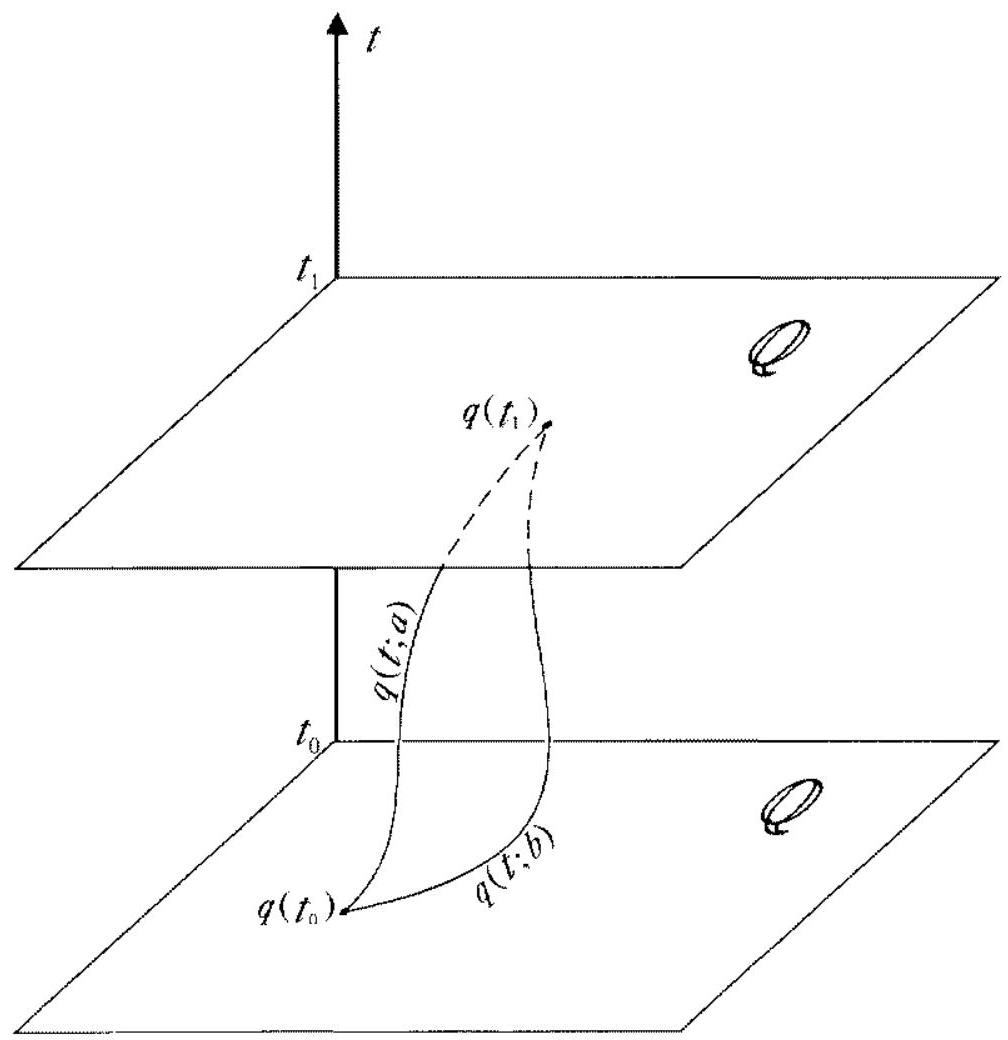
\includegraphics{variprin.jpg}
  \caption[]{Dos trayectorias posibles $ q(t ; a) $ y $ q(t ; b) $ desde $ q\left(t_{0}\right) $ hasta $ q\left(t_{1}\right) $. Los planos horizontales representan $ Q $ en los dos tiempos. Una familia continua de trayectorias posibles formaría una superficie en este diagrama, cuyas fronteras podrían ser $ q(t ; a) $ y $ q(t ; b) $.}
  \labfig{fig:}
\end{marginfigure}
\subsection{Ecuaciones de Euler-Lagrange}
Ahora procedemos a mostrar que la trayectoria física es la que da el valor mínimo de $ S $: minimizar $ S $ lleva a las ecuaciones de Lagrange. Consideremos una familia de muchas trayectorias $ q(t ; \epsilon) $, todas comenzando y terminando en $ q\left(t_{0}\right) $ y $ q\left(t_{1}\right) $, donde $ \epsilon $ es un índice que etiqueta cada trayectoria particular de la familia. Así como $ q(t ; a) $ y $ q(t ; b) $ conducen a diferentes acciones, cada $ q(t ; \epsilon) $ lleva a su correspondiente acción $ S(\epsilon) $. Entonces, el principio variacional establece que la trayectoria física es aquella para la cual la acción es un mínimo y que esto es independiente de la forma en que se elija la familia de trayectorias $ \epsilon $, siempre que contenga la física. Este es conocido como el principio variacional de Hamilton.

Más específicamente, requerimos que $ \epsilon $ tome sus valores de los números reales y parametrice la familia de trayectorias de forma continua y diferenciable. Esto significa que la familia forma una superficie conectada en el diagrama de la Fig. 3.1 y que la derivada parcial $ \partial q(t ; \epsilon) / \partial \epsilon $ existe para todos los valores de $ t $ en el intervalo $ \left[t_{0}, t_{1}\right] $. Todos los cálculos dependerán de $ \epsilon $ solo a través de derivadas, por lo que $ \epsilon $ puede cambiarse sin pérdida de generalidad agregando una constante arbitraria, y lo elegimos de manera que $ \epsilon=0 $ etiqueta la trayectoria que da el mínimo $ S $ en esa familia. (Por cierto, el requisito de diferenciabilidad se usará, y por lo tanto es necesario, solo en $ \epsilon=0 $.)

Las familias de trayectorias $ \epsilon $ se eligen de otra manera de manera bastante arbitraria, y solo por casualidad alguna de ellas contiene la trayectoria física. Sin embargo, en cualquier familia de este tipo, ya sea que incluya la trayectoria física o no, habrá una trayectoria para la cual $ S $ sea un mínimo. Esa trayectoria también puede incluirse en muchas otras familias $ \epsilon $, pero en general no dará el mínimo $ S $ en cada otra familia. Lo que el principio de Hamilton establece es que la trayectoria física da el mínimo $ S $ de cada familia en la que puede ser incluida. Matemáticamente, esto significa que para cualquier familia $ \epsilon $ tal, la trayectoria física satisface la ecuación

\begin{equation*}
\left.\frac{d S}{d \epsilon}\right|_{\epsilon=0} \equiv\left[\frac{d}{d \epsilon} \int_{t_{0}}^{t_{1}} L(q, \dot{q}, t) d t\right]_{\epsilon=0}=0 \tag{3.2}
\end{equation*}


A partir de ahora, abreviaremos $ d /\left.d \epsilon\right|_{\epsilon=0} $ como $ \delta $, por lo que (3.2) se convierte en

\begin{equation*}
\delta S \equiv \delta \int_{t_{0}}^{t_{1}} L(q, \dot{q}, t) d t=0 \tag{3.3}
\end{equation*}


Cabe recordar que en todas estas expresiones, todo se evalúa en $ \epsilon=0 $.

El siguiente paso es tomar la derivada de la integral con respecto a $ \epsilon $. La dependencia de $ \epsilon $ surge porque $ q $ y $ \dot{q} $ en el lagrangiano dependen de $ \epsilon $, así que

\begin{equation*}
\delta S=\int_{t_{0}}^{t_{1}} \delta L d t \tag{3.4}
\end{equation*}


Dado que $ \delta \equiv d /\left.d \epsilon\right|_{\epsilon=0} $,

\begin{equation*}
\delta L=\frac{\partial L}{\partial q^{\alpha}} \delta q^{\alpha}+\frac{\partial L}{\partial \dot{q}^{\alpha}} \delta \dot{q}^{\alpha} \tag{3.5}
\end{equation*}

Ahora, $ \dot{q}^{\alpha} \equiv \frac{d q^{\alpha}}{d t} $ es la velocidad generalizada a lo largo de una trayectoria especificada por un cierto valor de $ \epsilon $; es decir, la derivada temporal se toma para un $ \epsilon $ fijo. Esto debería escribirse como $ \frac{\partial q^{\alpha}}{\partial t} $, en lugar de $ \frac{d q^{\alpha}}{d t} $, pero en consonancia con la tradición y con la resolución final del problema, continuamos usando $ \frac{d q^{\alpha}}{d t} $. Dado que se trata de una derivada parcial, no hay problema en cambiar el orden de $ \frac{d}{d t} $ y $ \frac{\partial}{\partial \epsilon} $, y, por tanto, el orden de $ \frac{d}{d t} $ y $ \delta $. Así, tenemos

$$
\begin{aligned}
\frac{\partial L}{\partial \dot{q}^{\alpha}} \delta \dot{q}^{\alpha} & =\frac{\partial L}{\partial \dot{q}^{\alpha}} \frac{d}{d t} \delta q^{\alpha} \\
& =\frac{d}{d t}\left[\frac{\partial L}{\partial \dot{q}^{\alpha}} \delta q^{\alpha}\right]-\left[\frac{d}{d t} \frac{\partial L}{\partial \dot{q}^{\alpha}}\right] \delta q^{\alpha}
\end{aligned}
$$

Al insertar esto en la expresión para $ \delta L $, obtenemos


\begin{equation*}
\delta L=\left[\frac{\partial L}{\partial q^{\alpha}}-\frac{d}{d t} \frac{\partial L}{\partial \dot{q}^{\alpha}}\right] \delta q^{\alpha}+\frac{d}{d t}\left[\frac{\partial L}{\partial \dot{q}^{\alpha}} \delta q^{\alpha}\right] \tag{3.6}
\end{equation*}


Para un uso posterior, observamos que este resultado se obtuvo sin ninguna restricción sobre la variación de $ q(t, \epsilon) $ en los puntos finales.

Ahora, insertemos (3.6) en (3.4). Entonces,


\begin{equation*}
0=\delta S=\int_{t_{0}}^{t_{1}}\left[\frac{\partial L}{\partial q^{\alpha}}-\frac{d}{d t} \frac{\partial L}{\partial \dot{q}^{\alpha}}\right] \delta q^{\alpha} d t+\int_{t_{0}}^{t_{1}} \frac{d}{d t}\left[\frac{\partial L}{\partial \dot{q}^{\alpha}} \delta q^{\alpha}\right] d t \tag{3.7}
\end{equation*}


[Este resultado también podría haberse obtenido al insertar la Ec. (3.5) en la Ec. (3.4) e integrar el segundo término por partes.] El segundo integral aquí se obtiene fácilmente: es

$$
\left.\frac{\partial L}{\partial \dot{q}^{\alpha}} \delta q^{\alpha}\right|_{t_{1}}^{t_{1}}=0
$$

lo cual se anula porque en los puntos finales todas las trayectorias convergen, de modo que allí $ \delta q^{\alpha}=0 $. El término restante puede escribirse (ver Sección 2.2.2 para la definición de $ \Lambda_{\alpha} $):


\begin{equation*}
\int_{t_{0}}^{t_{1}} \Lambda_{\alpha} \delta q^{\alpha} d t=0 \tag{3.8}
\end{equation*}


Ahora, usemos el siguiente teorema (Gel'fand y Fomin, 1963). Sea $ f_{\alpha}, \alpha=1,2,\ldots,n $, un conjunto de $ n $ funciones integrables de una variable real $ t $ en un intervalo $ I $. Supongamos que


\begin{equation*}
\int_{I} f_{\alpha} h_{\alpha} d t=0 \tag{3.9}
\end{equation*}


para cualquier conjunto arbitrario de funciones integrables $ h_{\alpha} $ en el mismo intervalo, todas las cuales se anulan en sus puntos finales; entonces $ f_{\alpha}=0 $ para todos $ \alpha $. Dado que el principio de Hamilton se aplica a cualquier familia de trayectorias $ \epsilon $, los $ \delta q^{\alpha} $ son un conjunto de funciones arbitrarias de $ t $, al igual que los $ h_{\alpha} $, que se anulan en los puntos finales (recuerde que todo se evalúa en $ \epsilon=0 $). Por lo tanto, $ \Lambda_{\alpha}=0 $, o


\begin{equation*}
\frac{\partial L}{\partial q^{\alpha}}-\frac{d}{d t} \frac{\partial L}{\partial \dot{q}^{\alpha}}=0 \tag{3.10}
\end{equation*}


Estas son, por supuesto, las ecuaciones de Lagrange. Lo que nos dicen es que las funciones $ q^{\alpha}(t) $ que minimizan la acción, cuando se insertan junto con sus derivadas en la función lagrangiana y sus derivadas, son las mismas que satisfacen la ecuación de Lagrange.

En la Sección 3.2.2 será útil ver la Ec. (3.9) como un producto interno en un espacio vectorial $ \mathbb{F} $. Pensemos en los $ f_{\alpha} $ como los componentes de un vector $ f \in \mathbb{F} $ (y de manera similar $ h $), y escribamos

$$
\int_{I} f_{\alpha} h_{\alpha} d t \equiv(f, h)
$$

Entonces, el teorema citado arriba establece que si $ f $ es ortogonal a todos los vectores (arbitrarios $ h_{\alpha} $) en $ \mathbb{F} $, entonces $ f=0 $. Hay algunos puntos finos que podrían hacerse más rigurosos, pero esto será suficiente para nuestros propósitos. La derivación de las ecuaciones de Lagrange puede entonces expresarse en estos términos: la Ec. (3.8) establece que


\begin{equation*}
(\Lambda, \delta q)=0 \tag{3.11}
\end{equation*}


y dado que los $ \delta q $ son vectores arbitrarios y abarcan $ \mathbb{F} $, el vector $ \Lambda $ es ortogonal a todos los vectores en el espacio y, por lo tanto, se anula, que es el contenido de (3.10).
\subsection{Características de la acción}
garay

La acción de un sistema dinámico cuyas ecuaciones de movimiento son conocidas se construye de forma que estas se recuperen mediante el principio variacional. Sin embargo, la utilidad de este principio se debe a que, en muchos casos, es posible construir una acción para el sistema dinámico en cuestión mediante otras consideraciones (de simetría, por ejemplo), sin necesidad de conocer las ecuaciones de movimiento a priori.

He aquí algunas consideraciones ad hoc que se pueden tener en cuenta al construir la acción de un sistema dinámico:
\begin{itemize}
  \item La acción tiene dimensiones de momento angular.
  \item Consideraremos solo acciones locales en el tiempo. Por ejemplo, no consideraremos términos en la acción de la forma $\int \mathrm{d} t \mathrm{~d} t^{\prime} f\left(t, t^{\prime}\right) q(t) q\left(t^{\prime}\right)$.
  \todo{Esto es por la causalidad}
  \item Debe ser un funcional en el espacio de fases en velocidades $T \mathscr{Q}$. Podrían contener términos lineales en las segundas derivadas, pero mediante integración por partes, estos términos se pueden escribir como términos que dependen solo de primeras derivadas más términos que dependen de las condiciones iniciales y finales que no afectan a las ecuaciones de movimiento . Por ejemplo, la partícula libre se puede describir mediante la acción $S=\int \mathrm{d} t \delta_{i j} x^{i} \ddot{x}^{j}$, como es fácil comprobar . Esto es precisamente lo que ocurre cuando se añaden al lagrangiano derivadas totales $\dot{f}(q, \dot{q}, t)$ de funciones en el espacio de fases en velocidades ( $y$ no solo en el espacio de configuración), situación que no consideraremos aquí. Los sistemas con ecuaciones de evolución que contienen derivadas superiores tienen, salvo en situaciones concretas como la que acabamos de describir, comportamientos acausales.
  \item Si pretendemos describir sistemas con invariancias bajo ciertas transformaciones - simetrías-, es conveniente, pero no necesario, que la acción sea invariante bajo estas transformaciones. Por ejemplo, el segundo lagrangiano de la ecuación 1.2 describe la partícula libre, que es invariante bajo rotaciones, a pesar de que él mismo no lo sea.
  \item Para sistemas conservativos, la forma típica del lagrangiano es la diferencia entre la energía cinética y la potencial
  \begin{DispWithArrows}[format=c, displaystyle]
  L=T-V
  \end{DispWithArrows}
  , como se puede deducir a partir del principio de los trabajos virtuales y del principio de d'Alembert.
\end{itemize}

\subsection{Ligaduras}(114) (49-50) 

Las ligaduras aparecen en la dinámica cuando hay ciertas restricciones del movimiento. Miremos el siguiente ejemplo 
\begin{example}[Ejemplo ligaduras]
  Pensemos en una esfera que rueda sobre una superficie curva bajo la acción de la gravedad. La esfera está formada por muchas partículas cuyo movimiento está correlacionado, de modo que siempre forman una esfera rígida y siempre hay una de ellas en contacto con la superficie y, al rodar el cuerpo, instantáneamente en reposo. Las fuerzas que actúan sobre la esfera distan mucho de ser simples. Están compuestas por las fuerzas internas a la esfera (que la mantienen rígida), las fuerzas que le aplica la superficie sobre la que rueda (que la mantienen en contacto con dicha superficie y evitan que se deslice) y la fuerza de la gravedad. La fuerza de la gravedad se conoce a priori, pero las demás, las fuerzas de coacción, no. Lo que sí se sabe es que, bajo la acción de la gravedad y de las fuerzas de coacción, el cuerpo permanece sobre la superficie y sigue rodando. Podría parecer que para describir completamente el movimiento habría que encontrar las fuerzas de coacción, pero se demostrará lo contrario, que el movimiento puede obtenerse a partir de la fuerza gravitatoria y del conocimiento de las coacciones geométricas (es decir, de la forma de la superficie y del hecho de la rigidez); las fuerzas de coacción, si son necesarias, son más fáciles de encontrar después. Este ejemplo aparentemente sencillo de una esfera que rueda sobre una superficie curva es, en realidad, bastante complicado. La mayoría de las veces nos enfrentaremos a restricciones mucho más sencillas.
\end{example}

Hay dos tipos de ligaduras las cuales se definen de la siguiente manera:

\begin{definition}[Ligaduras Holonomas]
  Las ligaduras holónomas son aquellas que se pueden escribir mediante igualdades que involucran solo las variables de configuración y, quizá, el tiempo.
\end{definition}

\begin{definition}[Ligaduras Anholónomas]
  Las ligaduras anholónomas son aquellas que limitan el recorrido de las variables de configuración mediante desigualdades, que involucran las velocidades de forma que no se puedan transformar en otras que no las contengan o que, en general, no son holónomas.
\end{definition}



El método variacional de la Sección 3.1.1 seleccionó, entre todas las trayectorias que conectan $q\left(t_{0}\right)$ y $q\left(t_{1}\right)$, aquella que minimiza $S$. Sin embargo, este método debe ser modificado si el sistema está sujeto a restricciones, ya que las únicas trayectorias disponibles son aquellas que satisfacen las restricciones. Supongamos, por lo tanto, que el sistema está sujeto a $K<n$ restricciones independientes, en general no holonómicas (dependientes de la velocidad), de la forma

\begin{DispWithArrows}[displaystyle, format=c]
f_{I}(q, \dot{q} \cdot t)=0, \quad I=1,2, \ldots, K
\end{DispWithArrows}


Procedemos a aplicar el método variacional, ahora exigiendo que las trayectorias de comparación (las trayectorias entre las cuales se debe seleccionar la física) satisfagan las restricciones.

Comenzamos con la Ecuación (3.11), excepto que ahora $\delta q \in \mathbb{F}$, cuyos componentes son $\partial q^{\alpha} / \partial \epsilon$, no es arbitraria, ya que proviene de trayectorias $q(t ; \epsilon)$ que están restringidas por las Ecuaciones (3.12). La Ecuación (3.11) ahora dice que $\Lambda$ no es el vector nulo, sino que es ortogonal al subespacio $\mathbb{F}_{q} \subset \mathbb{F}$ generado por los $\delta q$ admisibles. Para encontrar las posibles $\Lambda$, debemos encontrar $\mathbb{F}_{q}$.

El subespacio $\mathbb{F}_{q}$ puede ser encontrado estableciendo con precisión cómo las Ecuaciones (3.12) restringen los vectores $\delta q$. Comencemos tomando las derivadas de las Ecuaciones (3.12) con respecto a $\epsilon$:

\begin{DispWithArrows}[displaystyle, format=c]
\frac{\partial f_{I}}{\partial \epsilon} \equiv \frac{\partial f_{I}}{\partial q^{\alpha}} \frac{\partial q^{\alpha}}{\partial \epsilon}+\frac{\partial f_{I}}{\partial \dot{q}^{\alpha}} \frac{\partial \dot{q}^{\alpha}}{\partial \epsilon}=0
\end{DispWithArrows}


Ahora multiplica cada una de estas ecuaciones por una función suficientemente bien comportada $\mu_{I}(t)$ y suma sobre $I$ (todas las sumas sobre $I$ están indicadas por signos de suma):

\begin{DispWithArrows}[displaystyle, format=c]
\int_{t_{0}}^{t_{1}} \sum_{l}\left[\mu_{l} \frac{\partial f_{l}}{\partial q^{\alpha}} \frac{\partial q^{\alpha}}{\partial \epsilon}+\mu_{l} \frac{\partial f_{l}}{\partial \dot{q}^{\alpha}} \frac{\partial \dot{q}^{\alpha}}{\partial \epsilon}\right] d t=0
\end{DispWithArrows}


Integra por partes, como en la derivación de la Ecuación (3.7), para obtener

\begin{DispWithArrows}[displaystyle, format=c]
\int_{t_{i}}^{l_{1}} \sum_{i}\left[\mu_{i} \frac{\partial f_{l}}{\partial q^{\alpha}}-\frac{d}{d t}\left(\mu_{1} \frac{\partial f_{l}}{\partial \dot{q}^{\alpha}}\right)\right] \frac{\partial q^{\alpha}}{\partial \epsilon} d t \equiv\left(\sum_{l} \chi_{l}, \delta q\right)=0
\end{DispWithArrows}

donde cada $\chi_{l}$ es el vector cuyas componentes son (sin suma sobre $I$)

\begin{DispWithArrows}[displaystyle, format=c]
\chi_{1 \alpha} \equiv \mu_{I} \frac{\partial f_{I}}{\partial q^{\alpha}}-\frac{d}{d t}\left(\mu_{I} \frac{\partial f_{I}}{\partial \dot{q}^{\alpha}}\right)
\end{DispWithArrows}


La Ecuación (3.14) da las restricciones sobre los vectores $\delta q$: son ortogonales a todos los posibles vectores $\chi_{I}$. El subespacio $\mathbb{F}_{4}$ que generan es ortogonal al subespacio $\mathbb{F}_{\chi} \subset \mathbb{F}$ generado por los $\chi_{1}$. (No hemos probado que ni $F_{4}$ ni $\mathbb{F}_{x}$ son subespacios, pero dejemos eso de lado).

Dado que $\Lambda$ es ortogonal a $\mathbb{F}_{q}$, que a su vez es ortogonal a $\mathbb{F}_{\chi}$, debe estar en $\mathbb{F}_{\chi}$. Es decir, existen constantes $\alpha_{1}$ tales que $\Lambda=\sum \alpha_{1} \chi_{1}$. Estos $\alpha_{1}$ pueden ser absorbidos en los $\mu_{1}$, escribiendo $\lambda_{I}(t)=\alpha_{I} \mu_{I}(t)$, y luego la definición de los $\Lambda_{\alpha}$ y la Ecuación (3.14) permiten que el resultado se exprese en la forma

\begin{DispWithArrows}[displaystyle, format=c]
\frac{d}{d t} \frac{\partial}{\partial \dot{q}^{\alpha}}\left(L+\sum \lambda_{l} f_{I}\right)-\frac{\partial}{\partial q^{\alpha}}\left(L+\sum \lambda_{l} f_{l}\right)=0
\end{DispWithArrows}

(los $\lambda_{1}$ se llaman multiplicadores de Lagrange). Este es el resultado de aplicar el principio variacional con restricciones: produce un conjunto de ecuaciones que se asemejan a las ecuaciones de EL para el Lagrangiano

\begin{DispWithArrows}[displaystyle, format=c]
\mathcal{L}=L+\sum \lambda_{1} f_{l}
\end{DispWithArrows}



Ahora tenemos las ecuaciones de Euler-Lagrange (EL) $n$ (3.15) y las ecuaciones de restricción $K$ (3.12) de las cuales debemos encontrar las funciones $q^{\alpha}(t)$ y $\lambda_{I}(t)$, que suman un total de $n+K$. Pero hay un problema serio: las Eqs. (3.15) son ecuaciones diferenciales de primer orden para los $\lambda_{I}$, y una solución requiere conocer los valores iniciales $\lambda_{l}\left(t_{0}\right)$. Este requisito es poco físico, ya que significa que deben conocerse las fuerzas iniciales de restricción (ver Problema 1) o, equivalente, las iniciales $\ddot{q}^{\alpha}$. Por esta razón, el enfoque variacional directo debe ser rechazado.

Sin embargo, si las restricciones son holonómicas (si los $f_{l}$ no dependen de los $\dot{q}^{\alpha}$), las Eqs. (3.15) se convierten en


\begin{DispWithArrows}[displaystyle, format=c]
\frac{d}{d t} \frac{\partial L}{\partial \dot{q}^{\alpha}}-\frac{\partial}{\partial q^{\alpha}}\left(L+\sum \lambda_{1} f_{I}\right)=0 \tag{3.17}
\end{DispWithArrows}


o


\begin{DispWithArrows}[displaystyle, format=c]
\frac{d}{d t} \frac{\partial L}{\partial \dot{q}^{\alpha}}-\frac{\partial L}{\partial q^{\alpha}}-\sum \lambda_{1} \frac{\partial f_{l}}{\partial q^{\alpha}}=0 \tag{3.18}
\end{DispWithArrows}


las cuales no involucran derivadas temporales de los $\lambda_{1}$. Así, la dificultad se evita. Para las restricciones holonómicas, las (3.17) son las ecuaciones aceptadas, y dado que los $f_{l}$ son independientes de $\dot{q}^{\alpha}$, las ecuaciones pueden escribirse como


\begin{DispWithArrows}[displaystyle, format=c]
\frac{d}{d t} \frac{\partial \mathcal{L}}{\partial \dot{q}^{\alpha}}-\frac{\partial \mathcal{L}}{\partial q^{\alpha}}=0 \tag{3.19}
\end{DispWithArrows}


con el $\mathcal{L}$ de (3.16).  
¿Qué se debe hacer en el caso general, cuando los $f_{1}$ dependen de los $\dot{q}^{\alpha}$? Una pista se obtiene al volver a las restricciones holonómicas, tomar sus derivadas temporales y llamar a estas las nuevas restricciones:


\begin{DispWithArrows}[displaystyle, format=c]
\hat{f}_{1} \equiv \frac{d f_{1}}{d t}=\frac{\partial f_{1}}{\partial q^{\alpha}} \dot{q}^{a}=0 \tag{3.20}
\end{DispWithArrows}


Las $\hat{f}_{1}(q, \dot{q}, t)$ son ahora restricciones dependientes de la velocidad, y en términos de ellas, la Eqs. (3.18) se convierte en


\begin{DispWithArrows}[displaystyle, format=c]
\frac{d}{d t} \frac{\partial L}{\partial \dot{q}^{\alpha}}-\frac{\partial L}{\partial q^{\alpha}}-\sum \lambda_{1} \frac{\partial \hat{f}_{I}}{\partial \dot{q}^{\alpha}}=0 \tag{3.21}
\end{DispWithArrows}


Este resultado es generalmente aceptado para restricciones dependientes de la velocidad, incluso si las $\hat{f}_{1}(q, \dot{q}, t)$, a diferencia de las de (3.20), son no lineales en los $\dot{q}^{\alpha}$.

\begin{marginfigure}[]
  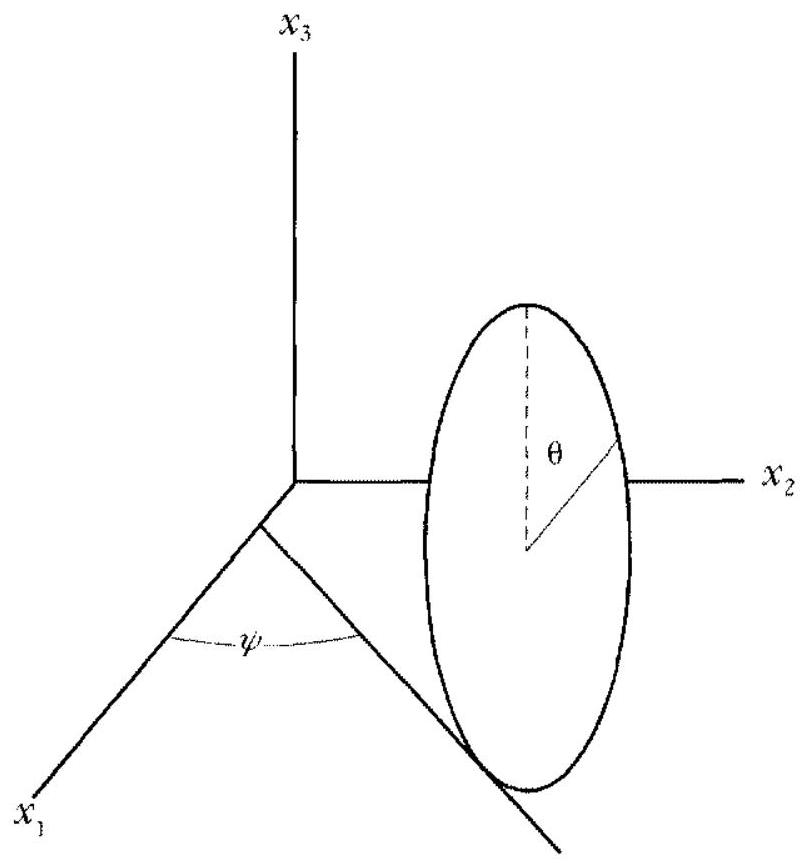
\includegraphics{exlig.jpg}
  \caption[]{Representación de las coordenadas generalizadas del ejemplo}
  \labfig{fig:exlig}
\end{marginfigure}

\begin{example}[Un disco de radio $R$ rueda sobre un plano horizontal perfectamente rugoso. (Esta es una restricción dependiente de la velocidad.) El disco está restringido a permanecer vertical. (Fig. 3.2) Escribe las ecuaciones de restricción y resuelve el movimiento en general.]
  


 La figura muestra las coordenadas generalizadas para este problema (las coordenadas del centro de masa del disco son $x_{1}$ y $x_{2}$). Las ecuaciones de restricción, que indican que el disco rueda, pueden escribirse como

$$
\begin{aligned}
& f_{1}=R \dot{\phi} \cos \psi-\dot{x}_{1}=0 \\
& f_{2}=R \dot{\phi} \sin \psi-\dot{x}_{2}=0
\end{aligned}
$$

El Lagrangiano es

$$
L=\frac{1}{2} I_{0} \dot{\phi}^{2}+\frac{1}{2} I_{1} \dot{\psi}^{2}+\frac{1}{2} m\left(\dot{x}_{1}^{2}+\dot{x}_{2}^{2}\right)
$$

donde $I_{0}$ es el momento de inercia del disco sobre su eje de simetría e $I_{1}$ es su momento de inercia sobre un diámetro. Las ecuaciones de movimiento son

$$
\Lambda_{\alpha}=\lambda_{I} \frac{\partial f_{I}}{\partial \dot{q}^{\alpha}}
$$

que, al desarrollarse, se convierten en

$$
\begin{align*}
& I_{0} \ddot{\phi}=\lambda_{1} R \cos \psi+\lambda_{2} R \sin \psi  \tag{3.22}\\
& I_{1} \ddot{\psi}=0  \tag{3.23}\\
& m \ddot{x}_{1}=-\lambda_{1}  \tag{3.24}\\
& m \ddot{x}_{2}=-\lambda_{2} \tag{3.25}
\end{align*}
$$

Las ecuaciones de restricción implican que $R \cos \psi=\dot{x}_{1} / \dot{\phi}$ y $R \sin \psi=\dot{x}_{2} / \dot{\phi}$, por lo que (3.22) se convierte en

$$
I_{0} \dot{\phi} \ddot{\phi}=\lambda_{1} \dot{x}_{1}+\lambda_{2} \dot{x}_{2}=-m\left(\dot{x}_{1} \ddot{x}_{1}+\dot{x}_{2} \ddot{x}_{2}\right)
$$

donde se han utilizado (3.24) y (3.25). Esto se integra inmediatamente para obtener

$$
I_{0} \dot{\phi}^{2}+m\left(\dot{x}_{1}^{2}+\dot{x}_{2}^{2}\right)=\text{constante}
$$

Pero las ecuaciones de restricción implican que $\dot{x}_{1}^{2}+\dot{x}_{2}^{2}=R^{2} \dot{\phi}^{2}$, por lo que $(I_{0}+m R^{2}) \dot{\phi}^{2}=\text{constante}$, o $\dot{\phi}=\text{constante}$. Así,

$$
\phi=\phi_{0}+\dot{\phi}_{0} t
$$

De (3.23) se sigue inmediatamente que

$$
\psi=\psi_{0}+\dot{\psi}_{0} t
$$

Insertando estos resultados en las ecuaciones de restricción e integrando se obtiene

$$
\begin{array}{ll}
\dot{x}_{1}=R \dot{\phi}_{0} \cos \left(\psi_{0}+\dot{\psi}_{0} t\right) ; & x_{1}=x_{10}+R \frac{\dot{\phi}_{0}}{\dot{\psi}_{0}} \sin \left(\psi_{0}+\dot{\psi}_{0} t\right) \\
\dot{x}_{2}=R \dot{\phi}_{0} \sin \left(\psi_{0}+\dot{\psi}_{0} t\right) ; & x_{2}=x_{20}-R \frac{\dot{\phi}_{0}}{\dot{\psi}_{0}} \cos \left(\psi_{0}+\dot{\psi}_{0} t\right)
\end{array}
$$

El disco rueda a una velocidad constante ($\dot{\phi}=\text{constante}$), cambiando de dirección también a una velocidad constante ($\dot{\psi}=\text{constante}$). Su centro de masa se mueve en un círculo de radio $\rho=\left|R \dot{\phi}_{0} / \dot{\psi}_{0}\right|$ centrado en $\left(x_{10}, x_{20}\right)$, para $\left(x_{1}-x_{10}\right)^{2}+\left(x_{2}-x_{20}\right)^{2}=\rho^{2}$. La velocidad del disco es constante, ya que $\dot{x}_{1}^{2}+\dot{x}_{2}^{2}=\left(R \dot{\phi}_{0}\right)^{2}=\text{constante}$.

Es evidente a partir de las Eqs. (3.24) y (3.25) que las $\lambda_{I}$ son las fuerzas que hacen que el disco se mueva de la manera en que lo hace. Estas son algunas de las fuerzas de restricción, ya que sin ellas el disco simplemente se movería en línea recta sobre el plano. Son solo algunas de las fuerzas de restricción porque hemos ignorado completamente las fuerzas que mantienen el disco vertical, tratando la masa como si estuviera toda concentrada en el punto de contacto sobre el plano y el disco como si no tuviera momento de inercia sobre el diámetro horizontal. Las componentes de las fuerzas de restricción en $x_{1}$ y $x_{}{2}$ son

$$
-\lambda_{1}=-R \dot{\phi}_{0} \dot{\psi}_{0} \sin \left(\psi_{0}+\dot{\psi}_{0} t\right), \quad-\lambda_{2}=R \dot{\phi}_{0} \dot{\psi}_{0} \cos \left(\psi_{0}+\dot{\psi}_{0} t\right)
$$

La fuerza de restricción es perpendicular a la velocidad (una fuerza centrífuga) y es proporcionada por la fricción con el plano. 

\end{example}


\section{Cantidades conservadas}(114-123)
\subsection{Coordenadas ciclicas}
A veces, las ecuaciones de Euler-Lagrange (EL) proporcionan una constante del movimiento de manera muy simple. Si una de las coordenadas generalizadas, digamos $q^{\beta}$, no aparece en el Lagrangiano (es una coordenada cíclica o ignorable), se cumple que $\partial L / \partial q^{\beta}=0$ y la ecuación EL de $\beta$ se expresa como


\begin{DispWithArrows}[displaystyle, format=c]
\frac{d}{d t} \frac{\partial L}{\partial \dot{q}^{\beta}}=0 
\end{DispWithArrows}


Esto implica claramente que $\partial L / \partial \dot{q}^{\beta}$ es una constante del movimiento. La función $p_{\beta}(q, \dot{q}, t)$ definida por


\begin{DispWithArrows}[displaystyle, format=c]
p_{\beta} \equiv \frac{\partial L}{\partial \dot{q}^{\beta}} 
\end{DispWithArrows}


se llama el momento generalizado conjugado a $q^{\beta}$. Si $q^{\beta}$ es ignorable\todo{Cuidad aquí que puede no aparecer en el Lagrangiano pero si en el extendido}, su momento conjugado $p_{\beta}$ proporciona un conjunto de subvariedades invariantes en $\mathbf{T Q}$. Es decir, si el punto de fase inicial se encuentra en alguna subvariedad cuya ecuación es de la forma $p_{\beta}=C$, el movimiento permanece en esa subvariedad.

Esto sugiere la utilidad de cambiar las coordenadas en $\mathbf{T} \mathbb{\sim}$ de $(q, \dot{q})$ a $(q, p)$. Más adelante, en la formulación hamiltoniana del Capítulo 5, haremos precisamente eso, pero implica pasar del haz tangente a otro conjunto llamado haz cotangente.

Supongamos, de manera más general, que alguna variable dinámica $\Gamma(q, \dot{q})$, que no necesariamente es uno de los $p_{\beta}$, se sabe que es constante en el movimiento. Su valor $C$ se determina por las condiciones iniciales $\Gamma\left(g_{0}, \dot{q}_{0}\right)=C$, y la ecuación $\Gamma(q, \dot{q})=C$ define una subvariedad invariantes de $(2 n-1)$ dimensiones (hiperficie) en $\mathbf{T Q}$. Cada $C$ diferente define una subvariedad invariante diferente, y las órbitas de fase yacen todas sobre tales subvariedades invariantes. Esto reduce el sistema dinámico de $2 n$ dimensiones en $\mathbf{T Q}$ a un conjunto de nuevos sistemas, cada uno de dimensión $2 n-1$ y cada uno etiquetado por su valor particular de $\Gamma$. De esta manera, cada constante del movimiento simplifica un sistema dinámico al reducir su dimensión en uno. Por esta razón, hay ventajas en encontrar sistemas de coordenadas con coordenadas ignorables: los momentos conjugados a los $q$ ignorables se conocen inmediatamente como constantes del movimiento.

Como ejemplo, nos dirigimos al Lagrangiano para el problema de fuerza central en el plano:


\begin{example}[Coordenadas cíclicas]


  \begin{DispWithArrows}[displaystyle, format=c]
    L=\frac{1}{2} \mu\left(\dot{r}^{2}+r^{2} \dot{\theta}^{2}\right)-V(r)
    \end{DispWithArrows}
    
    
    El ángulo $\theta$ es una coordenada ignorable, por lo que su momento conjugado, el momento angular $p_{\theta} \equiv \partial L / \partial \dot{\theta}$, se conserva. Cada una de sus subvariedades invariantes, dadas por
    
    
    \begin{DispWithArrows}[displaystyle, format=c]
    p_{\theta} \equiv \mu r^{2} \dot{\theta}=1
    \end{DispWithArrows}
    
    
    con diferentes valores $l$, define un nuevo sistema dinámico de un grado de libertad, como se discutió en la Sección 2.3.
\end{example}

Todo esto se puede expresar en términos de simetría, como se definió al comienzo de esta sección. Si $q^{\lambda}$ es ignorable, entonces $\partial L / \partial q^{\lambda}=0$, lo que significa que $L$ no cambia a medida que $q^{\lambda}$ varía, o $L$ es simétrico (o, como a menudo diremos, invariante) bajo la traducción en la dirección de $q^{\lambda}$ en $\mathbf{T Q}$.
\subsubsection{}
\subsection{Teorema de Noether}
\subsubsection{}
\subsubsection{}
\subsubsection{}

\section{Fuerzas disipativas}
(129-131)
\subsection{El oscilador harmónico amortiguado }


En previsión de los capítulos posteriores, nos dirigimos al ejemplo más conocido y sencillo de una fuerza proporcional a la velocidad, a saber, el oscilador armónico amortiguado. Comenzamos con un problema ligeramente más general para demostrar por qué el oscilador armónico surge con tanta frecuencia. Consideremos un sistema con un grado de libertad cuya Lagrangiana es
\begin{DispWithArrows}[displaystyle, format=c]
L=\frac{1}{2} \tau(q) \dot{q}^{2}-V(q) \tag{3.63}
\end{DispWithArrows}
donde $\tau$ es una función positiva definida (es decir, mayor que cero para todo $q$ ) y $V$ tiene un mínimo en algún valor $q_{0}$ de $q$. Para un pequeño desplazamiento $x$ desde $q_{0}$, el potencial $V$ se puede expandir en una serie de Taylor de la forma
$$
V(q)=V\left(q_{0}\right)+V^{\prime}\left(q_{0}\right) x+\frac{1}{2} V^{\prime \prime}\left(q_{0}\right) x^{2}+\frac{1}{6} V^{\prime \prime \prime}\left(q_{0}\right) x^{3}+\cdots
$$

Dado que $q_{0}$ es un mínimo para $V$, la primera derivada se anula. Toda función de energía potencial se define solo hasta una constante aditiva, la cual siempre se puede elegir para que $V\left(q_{0}\right)=0$; entonces la serie se convierte (cambiamos el argumento de $V$ de $q$ a $x$ )
\begin{DispWithArrows}[displaystyle, format=c]
V(x)=\frac{1}{2} k x^{2}+\frac{1}{6} s x^{3}+\cdots \tag{3.64}
\end{DispWithArrows}
donde $k \equiv V^{\prime \prime}\left(q_{0}\right)$ y $s \equiv V^{\prime \prime \prime}\left(q_{0}\right)$. Ahora expandimos también el término de energía cinética, nuevamente escribiendo todo en términos de $x$ (notar que $\dot{x}=\dot{q}$ ), para obtener
$$
\frac{1}{2} \tau(q) \dot{q}^{2}=\frac{1}{2} m \dot{x}^{2}+\frac{1}{2} r x \dot{x}^{2}+\cdots
$$
donde $m \equiv \tau\left(q_{0}\right)$ es positivo (bajo la suposición de que $\tau$ es una función positiva definida) y $r \equiv \tau^{\prime}\left(q_{0}\right)$. Entonces, si $k \neq 0$, para desplazamientos lo suficientemente pequeños desde el equilibrio, la Lagrangiana puede aproximarse por
\begin{DispWithArrows}[displaystyle, format=c]
L=\frac{1}{2} m \dot{x}^{2}-\frac{1}{2} k x^{2} \tag{3.65}
\end{DispWithArrows}
que es la Lagrangiana del oscilador armónico. En otras palabras, para vibraciones suficientemente pequeñas alrededor de un punto de equilibrio, todo sistema dinámico independiente del tiempo con un grado de libertad se comporta como un oscilador armónico, siempre que $V^{\prime \prime} \neq 0$ en el punto de equilibrio.

Si $V^{\prime \prime}\left(q_{0}\right)=0$ pero $V^{\prime \prime \prime}\left(q_{0}\right) \neq 0$, la fuerza es cuadrática en $x$ y, por lo tanto, siempre del mismo signo, siempre causando aceleraciones en la misma dirección. Entonces no es una fuerza restauradora y el equilibrio no es estable. De manera más general, para que ocurran oscilaciones, la potencia más baja en la expansión de Taylor del potencial debe ser par. Si $V^{\prime \prime \prime}\left(q_{0}\right)$ también se anula, el primer término en la expansión es cuártico y, aunque ocurren oscilaciones, el sistema es no lineal.

La Lagrangiana de la Ecuación (3.65) es la del oscilador armónico no amortiguado. Ahora añadimos una fuerza de amortiguación introduciendo la función de Rayleigh $\mathcal{F}=\hat{b} \dot{x}^{2}$. Entonces, de acuerdo con (3.60), la ecuación de movimiento es
\begin{DispWithArrows}[displaystyle, format=c]
m \ddot{x}+2 \hat{b} \dot{x}+k x=0 \tag{3.66}
\end{DispWithArrows}

Este es ahora el oscilador armónico amortiguado. Dos formas de su solución son
$$
\left.\begin{array}{l}
x(t)=e^{-\beta t}\left(A e^{t \omega t}+A^{*} e^{-t \omega t}\right)  \tag{3.67}\\
x(t)=e^{-\beta t}(a \cos \omega t+b \sin \omega t)
\end{array}\right\}
$$
donde $\beta=\hat{b} / m$ es el factor de amortiguación y $\omega=\sqrt{\omega_{0}^{2}-\beta^{2}}$, con $\omega_{0}=\sqrt{k / m}$. Las condiciones iniciales determinan las dos constantes reales de integración (ambas contenidas en la constante compleja $A$ en la primera forma y en $a$ y $b$ en la segunda).

Este sistema sigue siendo lineal, ya que $x$ y sus derivadas aparecen linealmente en la Ecuación (3.66). Si $V^{\prime \prime}\left(q_{0}\right)=0$ (como se mencionó anteriormente) o si la disipación no es proporcional a $\dot{x}$, es decir, si $\mathcal{F}$ no es cuadrática en $\dot{x}$, aparecerán algunas potencias superiores de $x$ y $\dot{x}$, lo que provocará que el sistema se vuelva no lineal. Los sistemas no lineales son considerablemente más complicados que los lineales. Serán discutidos con más detalle en el Capítulo 7.

El retrato de fase del oscilador no amortiguado (es decir, con $\beta=0$ ) se muestra en la Fig. 3.4. El retrato de fase consiste en elipses anidadas cuyas semiaxes son $c \equiv \sqrt{a^{2}+b^{2}}=|A|^{2}$ a lo largo del eje $x$ y $\omega c$ a lo largo del eje $\dot{x}$ (para el caso no amortiguado $\omega=\omega_{0}$ ). Cada elipse corresponde a un par de valores dados para $a$ y $b$, y la energía del movimiento está directamente relacionada con el área de la elipse (Problema 15).

Cuando $\beta \neq 0$, el retrato de fase consiste en curvas que convergen hacia el origen de $T \mathbb{Q}=\mathbb{R}^{2}$, como se muestra en la Fig. 3.5.

Si $\beta<\omega_{0}$, de modo que $\omega$ es real, las curvas son espirales, como la que se muestra en la Fig. 3.5(a), y el origen de $T \mathbb{Q}$ se llama el punto focal de la dinámica. El sistema oscila alrededor de $x=0$, con la amplitud disminuyendo en cada oscilación. Esto se llama el caso subamortiguado.

Si $\beta>\omega_{0}$, entonces $\omega \equiv i \nu$ es imaginaria y el sistema realiza como máximo una oscilación (dependiendo de las condiciones iniciales) antes de converger a $x=0$. Esto se llama el caso sobreamortiguado. Elige $v>0$ y observa que $\beta>v$. En términos de la constante real $v$,
$$
x(t)=e^{-\beta t}\left\{a e^{-\nu t}+b e^{v t}\right\}
$$


\section{Geometria}(134-136)

Una variedad diferenciable es, esencialmente, un conjunto de puntos que se puede describir por un atlas compuesto por mapas (a los que llamaremos cartas); una característica importante de un atlas es que las cartas que lo componen se deben superponer de forma suave. En este sentido, una variedad diferenciable es un conjunto de puntos que localmente se parece a $\mathbb{R}^{n}$.
\subsection{Campos vectoriales}

\begin{definition}[Vector tangente]
  Un vector tangente a una curva en un punto de una variedad diferenciable ( $y$, en particular, del espacio de fases) es un operador diferencial que asigna a cada función su derivada a lo largo de la curva. Más explícitamente, dada una curva $\gamma(s)$ parametrizada por $s$, definimos su vector tangente $\boldsymbol{X}$ como el operador que asigna a cada función $f$ el número
$$
X f=X(f):=\frac{\mathrm{d} f[\gamma(s)]}{\mathrm{d} s}=\frac{\mathrm{d} \gamma^{\alpha}}{\mathrm{d} s} \partial_{\alpha} f=\dot{\gamma}^{\alpha} \partial_{\alpha} f .
$$
\end{definition}

\begin{definition}[Campo vectorial]
  Un campo vectorial es una asignación suave de un vector a cada punto de la variedad. Los campos vectoriales son operadores diferenciales y, por tanto, son lineales y satisfacen la regla de Leibniz.
\end{definition}

Se define el conmutador de dos campos vectoriales $X$ y $Y$ como el campo vectorial
$$
[X, Y]=X Y-Y X=\left(X^{\alpha} \partial_{\alpha} Y^{\beta}-Y^{\alpha} \partial_{\alpha} X^{\beta}\right) \partial_{\beta}
$$
y satisface las siguientes propiedades:
\begin{itemize}
  \item linealidad, $\quad[a X+b Y, Z]=a[X, Z]+b[Y, Z] \quad \forall a, b \in \mathbb{R}$
  \item antisimetría, $[X, Y]=-[Y, X]$
  \item identidad de Jacobi, $\quad[X,[Y, Z]]+[Y,[Z, X]]+[Z,[X, Y]]=0$
\end{itemize}


Así, el conmutador dota al espacio tangente con la estructura de álgebra de Lie.
\subsection{Uno-formas}
\subsection{Ley de transformación I}
La ley de transformación de las componentes de un campo vectorial $X$ bajo un cambio arbitrario de coordenadas $\zeta^{\alpha} \rightarrow \zeta^{\prime \alpha}$ se deduce directamente de su definición:
$$
X^{\prime \alpha}=\frac{\partial \zeta^{\prime \alpha}}{\partial \zeta^{\beta}} X^{\beta}
$$
\subsection{Derivada de lie}
La derivada de Lie $\mathfrak{L}_{X}$ es un operador diferencial que da cuenta de cómo varían los campos tensoriales a lo largo de la curva generada por el campo vectorial $X$.

Dada una curva parametrizada por $s$ y cuyo vector tangente es $X$, podemos calcular cómo varía cualquier función a lo largo de la misma utilizando la definición de vector tangente: $\dot{f}=X f$. Por tanto,
$$
\dot{f}=\mathfrak{L}_{X} f=X f=X^{\alpha} \partial_{\alpha} f
$$

Notemos que, si la función $f$ tiene una dependencia explícita en el parámetro $s$, es necesario añadirla a esta expresión:
$$
\dot{f}=\mathfrak{L}_{X} f+\partial_{s} f=X f+\partial_{s} f
$$

La derivada de Lie de un campo vectorial $Y$ a lo largo de la curva generada por $X$ es un campo vectorial que tiene dos contribuciones, de acuerdo con la regla de Leibniz aplicada a la función $Y f$ para cualquier función $f$ :
$$
\mathfrak{L}_{X}(Y f)=\left(\mathfrak{L}_{X} Y\right) f+Y\left(\mathfrak{L}_{X} f\right)
$$

El primer miembro es la derivada de Lie de la función $Y^{\alpha} \partial_{\alpha} f$ y vale, por tanto, $X^{\beta} \partial_{\beta}\left(Y^{\alpha} \partial_{\alpha} f\right)$. Análogamente, el segundo término del segundo miembro se puede escribir de la forma $Y^{\beta} \partial_{\beta}\left(X^{\alpha} \partial_{\alpha} f\right)$. Concluimos así que
$$
\left(\mathfrak{L}_{X} Y\right) f=\left(X^{\beta} \partial_{\beta} Y^{\alpha}-Y^{\beta} \partial_{\beta} X^{\alpha}\right) \partial_{\alpha} f
$$
por lo que
$$
\mathfrak{L}_{X} Y=\left(X^{\beta} \partial_{\beta} Y^{\alpha}-Y^{\beta} \partial_{\beta} X^{\alpha}\right) \partial_{\alpha}=[X, Y]
$$

La primera contribución se debe a la manera en que cambian las componentes del campo $Y$ a lo largo de la curva. La segunda se debe a la propia evolución de los elementos de la base $\partial_{\alpha}$ a lo largo de la curva.

La derivada de Lie de una uno-forma $\boldsymbol{\sigma}$ es otra una uno-forma que se obtiene mediante el uso directo de la regla de Leibniz. La contracción $(\boldsymbol{\sigma}, Y)$ de $\boldsymbol{\sigma}$ con cualquier vector $Y$ involucra un producto tensorial y, además, es un escalar. Por tanto,
$$
\mathfrak{L}_{X}(\boldsymbol{\sigma}, Y)=\left(\boldsymbol{\sigma}, \mathfrak{L}_{X} Y\right)+\left(\mathfrak{L}_{X} \boldsymbol{\sigma}, Y\right)
$$

De esta expresión, obtenemos
$$
\mathfrak{L}_{X} \boldsymbol{\sigma}=\left(X^{\beta} \partial_{\beta} \sigma_{\alpha}+\sigma_{\beta} \partial_{\alpha} X^{\beta}\right) \mathrm{d} \zeta^{\alpha}
$$
\section{Variaciones temporales. Energía} (74)


\section{Partícula en un potencial}
Consideremos el lagrangiano de una partícula en un potencial
\begin{DispWithArrows}[displaystyle, format=c]
L=m \dot{\vec{x}}^{2} / 2-V(\vec{x}, t)
\end{DispWithArrows}
y estudiemos algunas posibles invariancias y sus cantidades conservadas correspondientes.
- Momento lineal. La acción es invariante bajo traslaciones infinitesimales constantes $\delta \vec{x}=\hat{n} \delta \epsilon$ en la dirección $\hat{n}$ o, en componentes, $\delta x^{i}=n^{i} \delta \epsilon$, si y solo si
\begin{DispWithArrows}[displaystyle, format=c]
\delta V=n^{i} \partial_{i} V \delta \epsilon=0
\end{DispWithArrows}
si y solo si $V$ no depende de la posición a lo largo de la dirección $\hat{n}$. En estas condiciones, el teorema de Noether nos garantiza que existe una cantidad conservada asociada:
\begin{DispWithArrows}[displaystyle, format=c]
\delta Q=p_{i} \delta x^{i}=n^{i} p_{i} \delta \epsilon
\end{DispWithArrows}
por tanto, el momento lineal $\hat{n} \cdot \vec{p}$ en la dirección $\hat{n}$ se conserva.
\begin{itemize}
  \item Momento angular. 
  
  La acción es invariante bajo rotaciones infinitesimales constantes $\delta \vec{x}=\hat{n} \times \vec{x} \delta \theta$ alrededor de una dirección $\hat{n}$ o, en coordenadas cartesianas, $\delta x^{i}=\epsilon^{i j k} n_{j} x_{k} \delta \theta$ si y solo si
  \begin{DispWithArrows}[displaystyle, format=c]
  \delta V=\epsilon^{i j k} n_{j} x_{k} \partial_{i} V \delta \theta=(\vec{x} \times \hat{n}) \cdot \vec{\nabla} V \delta \theta=0,
  \end{DispWithArrows}
  es decir, si y solo si $V$ es invariante bajo rotaciones alrededor de la dirección $\hat{n}$. En estas condiciones, el teorema de Noether nos garantiza que existe una cantidad conservada asociada:
  \begin{DispWithArrows}[displaystyle, format=c]
  \delta Q=p_{i} \delta x^{i}=p_{i} \epsilon^{i j k} n_{j} x_{k} \delta \theta=(\vec{x} \times \vec{p}) \cdot \hat{n} \delta \theta=\vec{L} \cdot \hat{n} \delta \theta ;
  \end{DispWithArrows}
  por tanto, el momento angular $\hat{n} \cdot \vec{L}$ en la dirección $\hat{n}$ se conserva.
  \item Energía. 
  
  La acción es invariante bajo traslaciones temporales infinitesimales constantes $\delta t=\delta \epsilon$ si y solo si
  \begin{DispWithArrows}[displaystyle, format=c]
  \delta V=\partial_{t} V \delta \epsilon=0
  \end{DispWithArrows}
  si y solo si $V$ es independiente del tiempo. En estas condiciones, el teorema de Noether nos garantiza que existe una cantidad conservada asociada:
  \begin{DispWithArrows}[displaystyle, format=c]
  \delta Q=\left[L-p_{i} \dot{x}^{i}\right] \delta t=-\left[m \dot{\vec{x}}^{2} / 2+V(\vec{x})\right] \delta \epsilon=-E \delta \epsilon
  \end{DispWithArrows}
  por tanto, la energía $E$ se conserva.
\end{itemize}
\section{Invariancia bajo reparametrizaciones temporales}
Supongamos que la acción de un sistema es invariante bajo reparametrizaciones temporales arbitrarias $t \rightarrow t^{\prime}=t+\delta t$ con $\delta t=\delta \epsilon(t)$. Entonces la cantidad conservada asociada es $\delta Q=-E \delta \epsilon(t)$. Puesto que $\delta \epsilon(t)$ es arbitrario y $\mathrm{d} \delta Q / \mathrm{d} t=0$, la única posibilidad es que la energía se anule. Esta es una característica general de los sistemas invariantes bajo reparametrizaciones temporales: la energía sobre trayectorias físicas se anula idénticamente.

Desde otro punto de vista, es interesante darse cuenta de que, bajo reparametrizaciones temporales, la acción de un sistema cambia en
\begin{DispWithArrows}[displaystyle, format=c]
\delta S=\int_{t_{1}}^{t_{2}} \mathrm{~d} t[(\delta \epsilon) L+\delta L]=\int_{t_{1}}^{t_{2}} \mathrm{~d} t\left[\left(L-\frac{\partial L}{\partial \dot{q}^{a}} \dot{q}^{a}\right)(\delta \epsilon)^{\cdot}+\frac{\partial L}{\partial t} \delta \epsilon\right] .
\end{DispWithArrows}

Para obtener esta expresión basta con tener en cuenta que, en este caso,
\begin{DispWithArrows}[displaystyle, format=c]
\delta L=\frac{\partial L}{\partial \dot{q}^{a}} \delta \dot{q}^{a}+\frac{\partial L}{\partial t} \delta t
\end{DispWithArrows}
hacer uso de la expresión 1.3 para $\delta \dot{q}$ y realizar algunas integraciones por partes . Por tanto, para que la acción sea invariante bajo reparametrizaciones temporales, es necesario y suficiente que el lagrangiano no dependa explícitamente del tiempo y que, además,
\begin{DispWithArrows}[displaystyle, format=c]
L-\frac{\partial L}{\partial \dot{q}^{a}} \dot{q}^{a}=0
\end{DispWithArrows}
condición necesaria y suficiente para que el lagrangiano sea homogéneo de grado 1 en $\dot{q}^{a}$. \todo{Esto es importante, ya que si tiene algún termino que sea $\propto \dot{q}^{a}\dot{q}^{b}$ (homogénea de grado 2 o superior), entonces la acción no será invariante }

Los sistemas invariantes bajo reparametrizaciones temporales son un ejemplo de una clase más general de sistemas lagrangianos con ligaduras, para los que no todas las ecuaciones de Euler-Lagrange son de segundo orden, es decir, son sistemas para los que $\operatorname{det}\left(\partial^{2} L / \partial \dot{q}^{a} \partial \dot{q}^{b}\right)=0$. Para verlo en este caso particular, basta con calcular la derivada con respecto a $\dot{q}^{b}$ de la expresión anterior y notar que las velocidades $\dot{q}^{a}$ son independientes.

Finalmente, notemos que, si elegimos un parámetro temporal específico que rompa la invariancia bajo reparametrizaciones, la energía ya no será nula y dependerá del parámetro elegido: el concepto de energía depende del parámetro temporal de evolución elegido, es decir, ;depende del reloj que utilicemos!
\begin{example}
  La acción
\begin{DispWithArrows}[displaystyle, format=c]
S=\pi_{0} \int \mathrm{~d} \sigma \sqrt{\frac{\dot{\vec{x}}^{2}}{}}
\end{DispWithArrows}
donde $\pi_{0}$ es una constante con dimensiones de momento lineal, $\sigma$ es un parámetro temporal arbitrario y $\stackrel{\rightharpoonup}{x}:=\mathrm{d} \vec{x} / \mathrm{d} \sigma$, es invariante bajo reparametrizaciones temporales, como se puede comprobar directamente o mediante el grado de homogeneidad del lagrangiano. Las ecuaciones de movimiento son 
\begin{DispWithArrows}[displaystyle, format=c]
\frac{\stackrel{\circ}{\vec{x}}}{\sqrt{\frac{\dot{x}^{2}}{2}}}=\hat{n}
\end{DispWithArrows}
donde $\hat{n}$ es un vector unitario constante. Vemos que esta partícula mantiene siempre un movimiento rectilíneo, pero el módulo de su velocidad no está determinado y, de hecho, es una función arbitraria del tiempo. Esta acción describe el movimiento de una partícula libre en términos de un tiempo arbitrario, no del tiempo absoluto empleado para definir los sistemas de referencia galileanos. La energía de esta partícula con respecto a este parámetro temporal arbitrario $\sigma$ es
\begin{DispWithArrows}[displaystyle, format=c]
E^{(\sigma)}=\frac{\stackrel{\circ}{x}}{\sqrt{\dot{\vec{x}}^2}} \cdot \frac{L}{\pi_0} .
\end{DispWithArrows}
\end{example}

\section{Simetrías gauge}
La invariancia bajo reparametrizaciones temporales es un ejemplo de simetría gauge. Las simetrías gauge permiten utilizar distintas descripciones matemáticas de la misma situación física (por ejemplo, distintas parametrizaciones temporales).

Las simetrías gauge se caracterizan porque desproveen parcialmente de significado físico a las variables de configuración: si la trayectoria $q(t)$ es una solución de las ecuaciones de Euler-Lagrange con unas ciertas condiciones iniciales $q(0)$ y $\dot{q}(0)$, entonces también lo será $q(t)+\delta q(t)$ con las mismas condiciones iniciales. Por ejemplo, en un sistema cuyo lagrangiano es invariante bajo reparametrizaciones temporales, si $q(t)$ es una solución con ciertas condiciones iniciales, también lo será cualquier trayectoria $q(t+\delta \epsilon(t))$ con las mismas condiciones iniciales. Así, tendremos clases de equivalencia de soluciones (relacionadas mediante transformaciones gauge) como trayectorias físicas.

Además, las cantidades Noether asociadas a las simetrías gauge son siempre nulas, lo que implica que tenemos ligaduras, es decir, que no todas las ecuaciones de Euler-Lagrange son de segundo orden, como hemos visto para el caso particular de la invariancia bajo reparametrizaciones. En efecto, en general, si tenemos una simetría gauge, entonces 
\begin{DispWithArrows}[displaystyle, format=c]
\delta Q=0.
\end{DispWithArrows}

Si derivamos esta expresión con respecto a $\dot{q}^{b}$, obtenemos la ecuación 
\begin{DispWithArrows}[displaystyle, format=c]
\frac{\partial^{2} L}{\partial \dot{q}^{a} \partial \dot{q}^{b}}\left(\delta q^{a}-\dot{q}^{a} \delta t\right)=0.
\end{DispWithArrows}

Puesto que las variaciones son obviamente independientes, podemos concluir que 
\begin{DispWithArrows}[displaystyle, format=c]
\operatorname{det}\left(\partial^{2} L / \partial \dot{q}^{a} \partial \dot{q}^{b}\right)=0.
\end{DispWithArrows}

Es importante notar la diferencia con las simetrías físicas, para las que las cantidades Noether conservadas no se anulan idénticamente. En este caso, la transformación caracterizada por $\delta q$, transforma una solución con unas condiciones iniciales $q(0)$ y $\dot{q}(0)$ en otra con otras condiciones iniciales $q(0)+\delta q(0)$ y $\dot{q}(0)+\delta \dot{q}(0)$. Por ejemplo, la invariancia bajo traslaciones $\delta q=\delta \epsilon$ relaciona una solución con condiciones iniciales $q(0)$ y $\dot{q}(0)$ en otra con condiciones iniciales $q(0)+\delta \epsilon$ y $\dot{q}(0)$; la invariancia bajo traslaciones temporales constantes $\delta t=\delta \epsilon$, la convierte en la solución con condiciones iniciales $q(\delta \epsilon)$ y $\dot{q}(\delta \epsilon)$.


\section{Dinámica Relativista}

Antes de empezar con la dinámica relativista y como parece que cuarto solo se da relatividad y calculo tensorial, es recomendable mirarse el apéndice de relatividad. 

\subsection{Accion}
Consideremos un conjunto de partículas relativistas descritas por sus posiciones espaciotemporales $x_{n}^{\mu}$ y sus correspondientes velocidades $\dot{x}_{n}^{\mu}$, donde el punto representa la derivada con respecto a su tiempo propio, y veamos cuál puede ser una posible acción para este sistema.

Si tuviésemos una sola partícula, una posible acción podría ser de la forma $S=\int \mathrm{d} \tau L\left(x^{\mu}, \dot{x}^{\mu}, \tau\right)$, donde $\tau$ es el tiempo propio de la partícula. Sin embargo, el cuadrado de la cuadrivelocidad tiene un valor fijo, $\dot{x}^{2}=-c^{2}$, es decir, el problema variacional correspondiente tiene una ligadura anholónoma que debemos introducir mediante un multiplicador de Lagrange siguiendo el procedimiento descrito en $\$ 1.1 .6$. Aún así, el tratamiento inadecuado de ignorar la ligadura y de proceder como si el sistema fuese libre proporciona el resultado correcto para una partícula libre o en interacción con un campo electromagnético.

Con más de una partícula, nos encontramos con la dificultad adicional de decidir para qué sistema $\tau$ es el tiempo propio. No parece razonable (aunque posible) elegir una partícula como privilegiada y plantear la evolución con respecto al tiempo propio de esa partícula concreta. Esto nos lleva a considerar acciones que no dependan del parámetro temporal que utilicemos, es decir, a considerar acciones invariantes bajo reparametrizaciones. Además, esta es una simetría que poseen las ecuaciones de movimiento.

En la construcción de una acción relativista, nos guiaremos por los siguientes criterios:

\begin{itemize}
  \item  Debe ser invariante bajo reparametrizaciones temporales.
\item  Debe ser invariante bajo transformaciones de Lorentz, para que sea independiente del sistema de referencia inercial escogido.
\item  En el límite no relativista y en ausencia de interacciones, debemos recuperar el lagrangiano $\sum_{n} m_{n} \vec{v}_{n}^{2} / 2$.
\end{itemize}

\subsubsection{Partículas libres}
Comencemos por definir la acción de un conjunto de partículas libres relativistas. La invariancia bajo reparametrizaciones temporales fuerza que el lagrangiano sea homogéneo en las velocidades y la invariancia Lorentz a que dependa de las velocidades a través de su cuadrado. Por tanto, el término de la acción correspondiente a la partícula $n$-ésima debe ser proporcional a 
\begin{DispWithArrows}[displaystyle, format=c]
\int \mathrm{d} \sigma \sqrt{-\grave{x}_{n}^{2}},
\end{DispWithArrows}
donde $\sigma$ es un parámetro temporal arbitrario y $\dot{x}=\mathrm{d} x / \mathrm{d} \sigma$. Este factor tiene dimensiones de longitud. Para que tenga dimensiones de acción, multiplicamos por $-m_{n} c$ donde $m_{n}$ es la masa de la $n$-ésima partícula. La razón para incluir el signo negativo será discutida en breve. Entonces podemos escribir la acción de un sistema de partículas libres como
\begin{DispWithArrows}[displaystyle, format=c]
S=\int \mathrm{d} \sigma\left[-\sum_{n} m_{n} c \sqrt{-\dot{x}_{n}^{2}}\right].
\end{DispWithArrows}

Puesto que $\dot{x}_{n}$ no es la cuadrivelocidad, no está sujeta a ninguna ligadura y puede ser variada libremente. En efecto, es fácil comprobar que $\grave{x}_{n}^{2}=-\left[c /\left(\mathrm{d} \sigma / \mathrm{d} \tau_{n}\right)\right]^{2}$ es libre ya que $\mathrm{d} \sigma / \mathrm{d} \tau_{n}$ es arbitraria, donde $\tau_{n}$ es el tiempo propio de la partícula $n$-ésima.

También podemos escribir esta acción, ya deparametrizada, en términos del tiempo $t$ correspondiente a un cierto sistema de referencia inercial. Para ello, elegimos como tiempo $\sigma$ el parámetro temporal $t$. En el instante $t$, las partículas se hallarán en la posición espaciotemporal $x_{n}^{\mu}=\left(c t, x_{n}^{i}\right)$ con respecto al sistema de referencia inercial elegido, por lo que
\begin{DispWithArrows}[displaystyle, format=c]
\dot{x}_{n}^{\mu}=\mathrm{d} x_{n}^{\mu} / \mathrm{d} t=\left(c, v_{n}^{i}\right), \quad \sqrt{-\dot{x}_{n}^{2}}=c \sqrt{1-\vec{v}_{n}^{2} / c^{2}}.
\end{DispWithArrows}

Por tanto, la acción también se puede escribir de la forma
\begin{DispWithArrows}[displaystyle, format=c]
S=-\sum_{n} m_{n} c^{2} \int \mathrm{~d} t \sqrt{1-\vec{v}_{n}^{2} / c^{2}}.
\end{DispWithArrows}

En el límite no relativista, podemos expandir esta acción en serie de potencias de la velocidad tridimensional de la $n$-ésima partícula $v_{n} / c$ :
\begin{DispWithArrows}[displaystyle, format=c]
\begin{aligned}
S & =-\sum_{n} m_{n} c^{2} \int \mathrm{~d} t\left[1-\frac{1}{2} \frac{\vec{v}_{n}^{2}}{c^{2}}+\mathscr{O}\left[\left(v_{n} / c\right)^{4}\right]\right] = \\
& =-\sum_{n} m_{n} c^{2} \int \mathrm{~d} t+\int \mathrm{d} t\left[\sum_{n} \frac{1}{2} m_{n} \vec{v}_{n}^{2}\right]+\mathscr{O}\left[\left(v_{n} / c\right)^{4}\right].
\end{aligned}
\end{DispWithArrows}

El primer término es constante (corresponde a una derivada total en el lagrangiano) y el segundo es la acción de un sistema de partículas libres no relativistas. Notemos que, si no hubiésemos introducido el signo negativo en $-m_{n} c$, habríamos obtenido la acción no relativista tradicional cambiada de signo.
\subsubsection{Partículas en un campo electromagenético}
Los campos electromagnéticos $\vec{E}$ y $\vec{B}$ están descritos por los potenciales escalar $\phi$ y vector $\vec{A}$, de forma que
$$
\vec{B}=\vec{\nabla} \times \vec{A}, \quad \vec{E}=-\vec{\nabla} \phi-\partial_{t} \vec{A} .
$$

Estos potenciales se pueden ver como las componentes temporal y espacial de un cuadrivector ${ }^{4} A^{\mu}=\left(\phi / c, A^{i}\right)$, en términos del cual, el campo electromagnético adquiere la forma

\begin{equation}
F_{\mu \nu}=\partial_{\mu} A_{\nu}-\partial_{\nu} A_{\mu} \tag{1.5}
\end{equation}


Obviamente, $F_{\mu \nu}$ es un tensor antisimétrico cuyas componentes son 
$$
F_{0 i}=-F_{i 0}=-E_{i} / c, \quad F_{i j}=\epsilon_{i j k} B^{k} .
$$

A la vista de la expresión 1.5 del campo electromagnético, dos potenciales $A_{\mu}$ y $A_{\mu}^{\prime}$ que se diferencien en $\partial_{\mu} f$, donde $f(x)$ es una función arbitraria de la posición espaciotemporal, determinan el mismo campo electromagnético .

La acción de un sistema de partículas en un campo electromagnético ha de ser, como ya hemos apuntado, invariante bajo reparametrizaciones temporales, invariante Lorentz y debe tener el límite no relativista adecuado. Además, como en el lagrangiano debe aparecer el potencial vector, la acción debe ser invariante bajo transformaciones gange $A_{\mu} \rightarrow A_{\mu}+\partial_{\mu} f$. Notemos que, en este tema, $A_{\mu}$ es un campo externo; por tanto, esta transformación gauge no es como las discutidas en $\$ 1.2 .6$, que involucran transformaciones de las variables dinámicas. Sí lo será en el tema 5 , cuando $A_{\mu}$ sea un campo dinámico cuya evolución debamos estudiar. Notemos por último que cada partícula interacciona con el campo electromagnético independientemente, es decir, que la acción será la suma de las acciones correspondientes a cada partícula, lo que nos permite estudiar cada partícula por separado.

Los únicos cuadrivectores de los que disponemos para construir la acción son $\grave{x}^{\mu} \mathrm{d} \sigma$ y $A^{\mu}$. Además, disponemos también del tensor métrico $\eta_{\mu \nu}$ y del psuedotensor de Levi-Civita $\varepsilon^{\mu \nu \rho \sigma}$. Los únicos invariantes Lorentz independientes que podemos construir con estos elementos son $A^{2}, \mathrm{~d} \sigma \dot{x}^{\mu} A_{\mu}$ y $\dot{x}^{2}(\mathrm{~d} \sigma)^{2}$. Así, el término más general invariante Lorentz e invariante bajo reparametrizaciones

\footnotetext{
${ }^{4}$ En este curso, no demostraremos esta afirmación.
}
deberá estar construido con estos elementos y deberá ser, además, homogéneo en las velocidades (para asegurar la invariancia bajo reparametrizaciones). Su forma más general es 
$$
\int \mathrm{d} \sigma \sqrt{-\dot{x}^{2}} H\left(A^{2}, \dot{x}^{\mu} A_{\mu} / \sqrt{-\dot{x}^{2}}\right)
$$
donde $H(x, y)$ es una función arbitraria. La invariancia de la acción bajo transformaciones gauge del campo electromagnético elimina todos los posibles términos salvo dos: $\int \mathrm{d} \sigma \sqrt{-\dot{x}^{2}}$ y $\int \mathrm{d} \sigma \dot{x}^{\mu} A_{\mu}$, correspondientes a $H(x, y)=1$ por un lado, y a $H(x, y)=y$ por el el otro .

Así, la acción de un sistema de partículas sometidas a un campo electromagnético externo será

\begin{equation}
S=\int \mathrm{d} \sigma L^{(\sigma)}=\sum_{n} \int \mathrm{~d} \sigma\left[-m_{n} c \sqrt{-\dot{x}_{n}^{2}}+q_{n} \dot{x}_{n}^{\mu} A_{\mu}\left(x_{n}\right)\right] 
\end{equation}

donde $q_{n}$ es la carga de la $n$-ésima partícula. Cuando sea necesario, como ocurre con el lagrangiano, especificaremos con el superíndice ${ }^{(\sigma)}$ la dependencia de la parametrización. Es fácil ver que esta acción tiene el límite no relativista correcto.
\subsection{Ecuaciones del movimiento}
Las ecuaciones del Euler-Lagrange correspondientes a la acción 1.6 de un sistema de partículas en un campo electromagnético son 
$$
\begin{aligned}
0=\frac{\delta S}{\delta x_{n}^{\mu}} & =\frac{\partial L^{(\sigma)}}{\partial x_{n}^{\mu}}-\frac{\mathrm{d}}{\mathrm{~d} \sigma} \frac{\partial L^{(\sigma)}}{\partial \dot{x}_{n}^{\mu}}= \\
& =-m_{n} c \frac{\mathrm{~d}}{\mathrm{~d} \sigma} \frac{\dot{x}_{n \mu}}{\sqrt{-\dot{x}_{n}^{2}}}+q_{n} \dot{x}_{n}^{\nu} F_{\mu \nu}\left(x_{n}\right) .
\end{aligned}
$$

Puesto que las partículas no interaccionan entre sí, podemos estudiar la evolución de cada una por separado en términos de su tiempo propio. La ecuación de evolución para cada una de ellas es entonces
$$
m_{n} \ddot{x}_{n \mu}=q_{n} \dot{x}_{n}^{\nu} F_{\mu \nu}\left(x_{n}\right) .
$$

Escogiendo $\sigma$ como el tiempo $t$ en un sistema de referencia inercial cualquiera, las componentes espacial y temporal de estas ecuaciones adquieren la forma 
$$
\frac{\mathrm{d}}{\mathrm{~d} t}\left(m_{n} \gamma_{n} \vec{v}_{n}\right)=q_{n}\left(\vec{E}+\vec{v}_{n} \times \vec{B}\right), \quad \frac{\mathrm{d}}{\mathrm{~d} t}\left(m_{n} \gamma_{n} c^{2}\right)=q_{n} \vec{v}_{n} \cdot \vec{E}
$$

La primera ecuación nos dice que la derivada temporal del momento cinético $m_{n} \gamma_{n} \vec{v}_{n}$ es igual a la fuerza de Lorentz. La segunda ecuación nos dice que el campo eléctrico realiza un trabajo empleado en cambiar la energía cinética $m_{n} \gamma_{n} c^{2}$ de cada partícula y que el campo magnético no realiza trabajo. Además, esta ecuación se puede reescribir de la forma 
$$
\frac{\mathrm{d}}{\mathrm{~d} t}\left(m_{n} \gamma_{n} c^{2}+q_{n} \phi\right)=q_{n}\left(\partial_{t} \phi-\vec{v}_{n} \cdot \partial_{t} \vec{A}\right)
$$

Por tanto, si el potencial vector $A^{\mu}=(\phi / c, \vec{A})$ es independiente del tiempo $x^{0}=c t$, entonces se conserva la energía de cada partícula $E_{n}=m_{n} \gamma_{n} c^{2}+q_{n} \phi\left(\vec{x}_{n}\right)$ correspondiente a este tiempo coordenado.
$\diamond$ EJERCICIO: Encontrar el límite no relativista de todos los resultados de esta sección.
\subsection{Cantidades Conservadas}
El teorema de Noether nos garantiza que, si la acción es invariante bajo una cierta transformación infinitesimal $\left(\delta x_{n}^{\mu}, \delta \sigma\right)$ que puede afectar tanto a las variables de configuración como al parámetro temporal, entonces existe una cantidad conservada dada por
$$
\delta Q=\sum_{n}\left[p_{n \mu} \delta x_{n}^{\mu}-E_{n}^{(\sigma)} \delta \sigma\right]
$$
donde
$$
p_{n \mu}=\partial L^{(\sigma)} / \partial \grave{x}_{n}^{\mu}, \quad E_{n}^{(\sigma)}=p_{n \mu} \dot{x}_{n}^{\mu}-L^{(\sigma)}
$$

Notemos que, por construcción, el cuadrimomento no depende de la parametrización. Para un sistema de partículas acopladas a un campo electromagnético,
$$
p_{n \mu}=m_{n} \frac{\dot{x}_{n \mu}}{\sqrt{-\dot{x}_{n}^{2}}}+q_{n} A_{n \mu}=m_{n} \dot{x}_{n \mu}+q_{n} A_{n \mu}
$$

Por otro lado, es fácil comprobar que la energía $E^{(\sigma)}$ asociada al tiempo arbitrario $\sigma$ de este sistema se anula, como debe ocurrir puesto que la acción 1.6 es invariante bajo reparametrizaciones temporales.
\subsubsection{Cuadrimomento}
Cuando la acción es invariante bajo traslaciones infinitesimales constantes (activas) en una dirección espaciotemporal $n^{\mu}$ que no afectan al parámetro temporal $\delta x_{n}^{\mu}=n^{\mu} \delta \epsilon$, la cantidad Noether conservada es la proyección del cuadrimomento conjugado total en esa dirección
$$
n^{\mu} P_{\mu}=n^{\mu} \sum_{n} p_{n \mu}
$$

Es importante notar que la cantidad que se conserva no es el momento cinético total $\sum_{n} m_{n} \dot{x}_{n}^{\mu}$ sino el cuadrimomento conjugado total. Para sistemas cuyo lagrangiano no tiene dependencia lineal en las velocidades, ambos obviamente coinciden.

Si $n^{\mu}$ es un vector espacial, existe un sistema de referencia inercial en el que $n^{0}=0$ y la cantidad conservada es obviamente el momento lineal (relativista) $\hat{n} \cdot \vec{P}$ en esa dirección y en ese sistema de referencia. Por ejemplo, para un sistema de partículas cargadas,
$$
\hat{n} \cdot \vec{P}=\hat{n} \cdot \sum_{n} \vec{p}_{n}, \quad \vec{p}_{n}=\gamma_{n} m_{n} \vec{v}_{n}+q_{n} \vec{A}\left(x_{n}\right)
$$

Si $n^{\mu}$ es un vector temporal, entonces existe un sistema de referencia inercial en el que $n^{\mu}=(1,0,0,0)$; la cantidad conservada correspondiente es la energía correspondiente a traslaciones temporales en ese sistema de referencia inercial
$$
c P^{0}=\sum_{n}\left[\gamma_{n} m_{n} c^{2}+q_{n} \phi\left(x_{n}\right)\right]
$$

Para que la acción 1.6, sea invariante bajo traslaciones en la dirección $n^{\mu}$, basta con que el potencial vector $A_{\mu}$ sea independiente de la posición en esa dirección, es decir, que $n^{\mu} \partial_{\mu} A_{\nu}=0$.
\subsubsection{Cuadrimomento angular}
Toda transformación de Lorentz se puede escribir como una composición de transformaciones de Lorentz infinitesimales $\Lambda^{\mu}{ }_{\nu}=\delta_{\nu}{ }^{\mu}+\delta \omega^{\mu}{ }_{\nu}$ (ver apéndice C). Una transformación de Lorentz infinitesimal (activa) de las posiciones adquiere la forma:
$$
\delta x_{n}^{\mu}=-\delta \omega^{\mu}{ }_{\nu} x_{n}^{\nu} .
$$

Si la acción es invariante bajo alguna de las transformaciones de Lorentz (de parámetros $\delta \omega^{\mu}{ }_{\nu}$ ), entonces existe una cantidad conservada asociada
$$
\begin{aligned}
\delta Q & =\sum_{n} p_{n \mu} \delta x_{n}^{\mu}=-\sum_{n} p_{n}^{\mu} x_{n}^{\nu} \delta \omega_{\mu \nu}= \\
& =\frac{1}{2} \sum_{n} l_{n}^{\mu \nu} \delta \omega_{\mu \nu}=\frac{1}{2} J^{\mu \nu} \delta \omega_{\mu \nu}
\end{aligned}
$$
donde $l_{n}^{\mu \nu}=x_{n}^{\mu} p_{n}^{\nu}-x_{n}^{\nu} p_{n}^{\mu}$ es el momento angular cuadridimensional de la partícula $n$-ésima y $J^{\mu \nu}=\sum_{n} l_{n}^{\mu \nu}$ es el cuadrimomento angular total.

Si separamos los boosts de las rotaciones espaciales, podemos reescribir esta expresión de la forma (ver apéndice C )
$$
\delta Q=\delta \vec{\theta} \cdot \vec{J}+\delta \vec{\zeta} \cdot \vec{K}
$$
donde
$$
\begin{aligned}
J^{i} & =\frac{1}{2} \epsilon^{i j k} J_{j k}, & \delta \theta^{i} & =\frac{1}{2} \epsilon^{i j k} \delta \omega_{j k}, \\
K_{i} & =J_{i 0}, & \delta \zeta_{i} & =\delta \omega_{0 i} .
\end{aligned}
$$

En particular, si la acción es invariante bajo rotaciones alrededor de una cierta dirección $\hat{n}$ parametrizadas por $\delta \vec{\theta}=\hat{n} \delta \theta$, entonces se conserva el momento angular total en esa dirección $\hat{n} \cdot \vec{j}$. Asimismo, si la acción es invariante bajo transformaciones de Lorentz puras a lo largo de una cierta dirección $\hat{n}$ parametrizadas por $\delta \vec{\zeta}=\hat{n} \delta v / c$, entonces se conserva la cantidad $\hat{n} \cdot \vec{K}$.

En presencia de un campo electromagnético, la invariancia de la acción 1.6 bajo transformaciones de Lorentz puras está garantizada; también lo está la invariancia bajo rotaciones alrededor de $\hat{n}$, si el potencial vector $A_{\mu}$ es independiente de la correspondiente coordenada angular.
\subsubsection{Centro de inercia}
Consideremos ahora un sistema de referencia inercial en el que las partículas, en el instante $x^{0}=c t$, se hallan en las posiciones $x_{n}^{i}$. Entonces definimos el centro de inercia como
$$
X^{i}=\sum_{n} x_{n}^{i} p_{n}^{0} / P^{0}
$$

Debe notarse que esta definición no es covariante y que, por tanto, depende del sistema de referencia inercial elegido. Sumando y restando $x^{0} P^{i} / P^{0}$, podemos reescribir la posición del centro de inercia de la siguiente manera:
$$
X^{i}=-K^{i} / P^{0}+x^{0} P^{i} / P^{0}
$$

Si el lagrangiano del sistema de partículas es invariante bajo transformaciones de Lorentz puras y bajo traslaciones temporales, tanto $K^{i}$ como $P^{0}$ son cantidades conservadas. Entonces vemos que $K^{i}$, las cantidades conservadas asociadas a la invariancia bajo transformaciones de Lorentz puras, se pueden interpretar como las posiciones iniciales del centro de inercia
$$
Y^{i}=-K^{i} / P^{0}
$$
en el sistema de referencia inercial escogido, que son cantidades conservadas equivalentes a las $K^{i}$. Si además la acción es invariante bajo traslaciones espaciales, $P^{i}$ también se conserva y el centro de inercia se mueve con velocidad $P^{i} / P^{0}$ constante.

Llamaremos sistema de referencia del centro de inercia a cualquier sistema de referencia inercial propio del centro de inercia, es decir, tal que $P^{i}=0$. Obviamente, la trayectoria del centro de inercia en un sistema del centro de inercia es $X^{i}=Y^{i}$.

Es posible dar una expresión covariante para estas cantidades conservadas. En efecto, el cuadrivector
$$
Y^{\mu}=\frac{1}{P \rho P_{\rho}} J^{\mu \nu} P_{\nu}
$$
adquiere la forma $Y_{\mathrm{CI}}^{\mu}=J^{\mu 0} P_{0} /\left.\left(P^{0} P_{0}\right)\right|_{\mathrm{CI}}=\left.\left(0,-K^{i} / P^{0}\right)\right|_{\mathrm{CI}}$ en un sistema del centro de inercia. Así, tenemos un cuadrivector que, en un sistema de referencia inercial dado, adquiere la forma $\left(0,-K^{i} / P^{0}\right)$, que es la posición espaciotemporal inicial del centro de inercia. Por tanto, el cuadrivector $Y^{\mu}$ proporciona una expresión covariante para la posición inicial del centro de inercia. Obviamente, las cuatro componentes de este vector son cantidades conservadas. Sin embargo, puesto que $Y^{\mu}$ es perpendicular a $P^{\mu}$, solo tres de ellas son independientes.
\subsubsection{Invariantes Casimir}
Si la acción es invariante bajo todo el grupo de transformaciones de Poincaré (traslaciones y transformaciones de Lorentz), el momento total $P^{\mu}$ y el momento angular total $J^{\mu \nu}$ se conservan en la evolución pero, obviamente, estos no son
invariantes bajo el grupo de Poincaré.



\begin{definition}[Invariantes Casimir]



  Los invariantes Casimir son cantidades conservadas que también son invariantes Poincaré, es decir, que son independientes del sistema de referencia inercial elegido y que, por tanto, caracterizan intrínsecamente al sistema desde el punto de vista dinámico.
\end{definition}

A cntinuación veamos algunos invariantes Casimir de algunas cantidades conocidas

\begin{example}[Momento lineal]


  El momento $P^{\mu}$ es un vector bajo transformaciones de Lorentz que, obviamente, es invariante bajo traslaciones (es decir, bajo cambios del origen de coordenadas). Por tanto, $P^{\mu} P_{\mu}$ es un invariante Poincaré que, además, es conservado. De hecho, nos proporciona la masa total del sistema o, al menos, una definición apropiada de la misma. En efecto, puesto que $P^{\mu} P_{\mu}$ es un invariante, podemos evaluarlo en cualquier sistema de referencia inercial. $P^{\mu}$ es el momento total del sistema y, por tanto, en cualquier sistema del centro de inercia, $P_{\mathrm{CI}}^{i}=0$ por definición. Por tanto, en cualquier sistema del centro de inercia,
$$
-P^{\mu} P_{\mu}=\left(P_{\mathrm{CI}}^{0}\right)^{2}=\left(\sum_{n} p_{n \mathrm{CI}}^{0}\right)^{2}:=m^{2} c^{2}
$$
\todo{Como es invariante nos vamos al sistema más sencillo que es el del centro de inercia}


donde $m$ es la masa total del sistema en el siguiente sentido:

\framedtext{Es el valor más bajo que puede tomar la energía en cualquier sistema de referencia inercial. En efecto, en cualquier otro sistema de referencia inercial, la energía total del sistema será \marginnote[-2.2cm]{
  \begin{kaobox}[frametitle=Recuerda]
    $P^\mu=(\frac{E}{c}P^i)$
\end{kaobox}
}$E=c P^{0}=\sqrt{m^{2} c^{4}+c^{2} P^{i} P_{i}}$, que es siempre mayor o igual que $m c^{2}$.}

Si escribimos esta ecuación en términos de la velocidad del centro de inercia $E=m c^{2} \sqrt{1+c^{-2} \gamma^{2} \vec{v}^{2}}$ y expandimos en serie, obtenemos
$$
E=m c^{2}+m \vec{v}^{2} / 2+O\left[(\vec{v} / c)^{4}\right]
$$
que es la expresión no relativista de la energía total (energía en reposo más energía cinética) de un sistema de partículas en ausencia de fuerzas externas en la mecánica de Newton.

\end{example}
Notemos que, si hemos incluido un posible campo electromagnético externo, la invariancia bajo traslaciones espaciotemporales exige que el potencial vector $A_{\mu}$ sea independiente de las coordenadas y que, por tanto, el campo electromagnético externo sea nulo.
\begin{example}[Pseudovector de Pauli-Lyubarskii]
  Consideremos ahora el pseudovector de Pauli-Lyubarskii
  $$
W^{\mu}=\frac{1}{2} \varepsilon^{\mu \nu \rho \sigma} P_{\nu} J_{\rho \sigma}
$$

Por definición, $W^{\mu}$ es ortogonal a $P^{\mu}$ y además es invariante bajo traslaciones. Por tanto, $W^{\mu} W_{\mu}$ es independiente de $P^{\mu} P_{\mu}$, es invariante Poincaré y es conservado. Veamos cuál es su interpretación física. Puesto que $W^{\mu} W_{\mu}$ es invariante, podemos evaluarlo en cualquier sistema de referencia inercial, en particular, en el cualquier sistema del centro de inercia del sistema. Puesto que, en cualquier sistema del centro de inercia, $P_{\mathrm{CI}}^{i}=0$,
$$
W_{\mathrm{CI}}^{\mu}=\frac{1}{2} \varepsilon^{\mu 0 \rho \sigma} P_{\mathrm{Cl} 0} J_{\mathrm{Cl} \rho \sigma}=\frac{1}{2} \varepsilon^{\mu 0 j k} P_{\mathrm{Cl} 0} J_{\mathrm{Cl} j k}=-\frac{1}{2}\epsilon^{0ijk}P_{CI0}
$$

\todo{Los términos antisimétricos se cancelan}
Así, vemos que
$$
W_{\mathrm{CI}}^{0}=0, \quad W_{\mathrm{CI}}^{i}=\frac{1}{2} P_{\mathrm{CI}}^{0} \epsilon^{i j k} J_{\mathrm{CI} j k}
$$
y, por tanto,
$$
W^{\mu} W_{\mu}=m^{2} c^{2} \vec{S}^{2}
$$
donde $S_{i}=\frac{1}{2} \epsilon_{i j k} J_{\mathrm{cI}}^{j k}$ es el momento angular del sistema de partículas en cualquier sistema del centro de inercia y recibe el nombre de espín.

En cualquier sistema del centro de inercia de un conjunto de partículas,
$$
S_{i}=\frac{1}{2} \epsilon_{i j k} J_{\mathrm{CI}}^{j k}=\epsilon_{i j k} \sum_{n} x_{n}^{j} p_{n}^{k}
$$

Este es el \underline{espín del sistema} y es \underline{intrínseco}: 

Solo depende de la configuración interna (posiciones y momentos lineales relativos de las partículas que lo componen). Que solo depende de los momentos lineales relativos y no del total es obvio puesto que $P_{\mathrm{CI}}^{i}=\sum_{n} p_{n}^{i}=0$. Que no depende del origen que se tome para calcular el momento angular y que, por tanto, solo depende de las posiciones relativas, es fácil de ver. En efecto, si desplazamos el origen de coordenadas en una cantidad $R^{i}$, entonces el espín definido con respecto al nuevo origen será
$$
S_{i}^{\prime}=\epsilon_{i j k} \sum_{n}\left(x_{n}^{j}+R^{j}\right) p_{n}^{k}=S_{i}+\epsilon_{i j k} \sum_{n} R^{j} p_{n}^{k}
$$
pero el último término se anula debido a que $\sum_{n} p_{n}^{i}=0$. Es decir, el espín solo depende de la configuración interna del sistema.

\end{example}

\begin{corollary}
  La masa total del sistema $m$ y su momento angular intrínseco $\vec{S}^{2}$ son las únicas cantidades conservadas e invariantes bajo el grupo de Poincaré independientes. Cualquier otra se puede escribir en términos de ellas. La demostración
  de esta afirmación se basa en que ambos son los casimires del grupo de Poincaré y no la presentaremos aquí.
  
  Si la masa es nula, entonces, además de la relación de ortogonalidad entre $W^{\mu}$ y $P^{\mu}, W^{\mu} P_{\mu}=0$, tenemos que $P^{\mu} P_{\mu}=W^{\mu} W_{\mu}=0 \mathrm{y}$, por tanto, los vectores $W^{\mu}$ y $P^{\mu}$ son proporcionales.
\end{corollary}


